%% =====================================================================
%% Informe final del proyecto de grado — Maestría en Inteligencia Artificial
%% Universidad de los Andes · Curso Proyecto: despliegue de soluciones
%% Plantilla: IEEEtran.cls v1.7a (modo conference), según el ejemplo
%% de la carpeta Ejemplo-Proyecto-LaTeX2e.
%%
%% Compilar:  pdflatex articulo.tex   (dos veces, para referencias cruzadas)
%%   o bien:  latexmk -pdf articulo.tex
%%
%% Los resultados que aún no existen están marcados con \pendiente{...}
%% (texto rojo). Antes de entregar: buscar "\pendiente" y reemplazar.
%% =====================================================================
\documentclass[conference,letterpaper]{IEEEtran}

% ---------- Codificación, idioma y tipografía ----------
\usepackage[T1]{fontenc}
\usepackage[utf8]{inputenc}
\usepackage{mathptmx}            % Times, como pide el formato del curso
% Español si está instalado babel-spanish; si no, se traducen los rótulos a mano.
\IfFileExists{spanish.ldf}{%
  \usepackage[spanish,es-tabla,es-nodecimaldot,es-noshorthands]{babel}%
}{%
  \usepackage[english]{babel}%
  \addto\captionsenglish{%
    \renewcommand{\figurename}{Figura}%
    \renewcommand{\tablename}{Tabla}%
    \renewcommand{\refname}{Referencias}%
    \renewcommand{\abstractname}{Resumen}}%
}
\usepackage{icomma}              % coma decimal en modo matemático
\usepackage{microtype}

% ---------- Matemáticas, tablas y figuras ----------
\usepackage{amsmath,amssymb}
\usepackage{graphicx}
\usepackage{booktabs}
\usepackage{multirow}
\usepackage{tabularx}
\usepackage{array}
\usepackage[table]{xcolor}
\usepackage{tikz}
\usetikzlibrary{arrows.meta,positioning,fit,backgrounds,calc,shapes.geometric}
\usepackage{pgfplots}
\pgfplotsset{compat=1.16}
\usepackage{cite}
\usepackage{url}
\usepackage[hidelinks]{hyperref}

% ---------- Formato del curso: secciones 1, 2, 3 y 2.1, 2.2 en negrita ----------
\renewcommand\thesection{\arabic{section}}
\renewcommand\thesubsection{\thesection.\arabic{subsection}}
\renewcommand\thesectiondis{\thesection.}
\renewcommand\thesubsectiondis{\thesection.\arabic{subsection}.}
\renewcommand\thesubsubsectiondis{\thesubsection.\arabic{subsubsection}.}
\makeatletter
\def\section{\@startsection{section}{1}{\z@}{1.6ex plus 1.2ex minus 0.4ex}%
  {0.8ex plus 0.4ex minus 0.2ex}{\normalfont\normalsize\bfseries}}
\def\subsection{\@startsection{subsection}{2}{\z@}{1.2ex plus 1ex minus 0.3ex}%
  {0.6ex plus 0.3ex minus 0.1ex}{\normalfont\normalsize\bfseries}}
\makeatother

% ---------- Utilidades del equipo ----------
% Marca de contenido pendiente: se ve en rojo y se busca con "\pendiente".
\newcommand{\pendiente}[1]{\textcolor{red}{\textbf{[Pendiente:} #1\textbf{]}}}
\newcommand{\fuente}[1]{\emph{Fuente: #1}}
\definecolor{tinta}{HTML}{1F4E52}
\definecolor{acento}{HTML}{D9694C}
\definecolor{niebla}{HTML}{EEF3F2}

\hyphenation{an-tro-po-mé-tri-cas o-xi-ge-no-de-pen-den-cia re-ad-mi-sión pre-ma-tu-ros
  se-gui-mien-to ca-li-bra-ción ex-pli-ca-ción ob-ser-va-to-rio pseu-do-ni-mi-za-da
  e-xi-gen-cia an-te-rior de-sen-la-ces di-ccio-na-rio ló-gi-ca pro-ba-bi-li-dad}

\begin{document}

\renewcommand{\abstractname}{Resumen}
\def\IEEEkeywordsname{Palabras clave}

\title{KMCPred: sistema interpretable de alertas y predicción temprana de riesgos en niños prematuros y de bajo peso del Programa Madre Canguro}

\author{%
\IEEEauthorblockN{Alex P. Chirino Caicedo, Breitner E. González Angarita,\\
Santiago J. Ramos Echeverry y Wilfrido A. Gómez Pérez}
\IEEEauthorblockA{Maestría en Inteligencia Artificial, Universidad de los Andes, Colombia\\
En colaboración con la Fundación Canguro\\
\{a.chirino, b.gonzalez, s.ramose, w.gomezp\}@uniandes.edu.co}}

\maketitle

\begin{abstract}
El seguimiento de niños prematuros y de bajo peso del Programa Madre Canguro produce registros clínicos que permiten estudiar la calidad de los datos y anticipar riesgos en el crecimiento y desarrollo infantil. Presentamos KMCPred, una plataforma de IA interpretable desarrollada con información del Observatorio Canguro: 62.043 niños y 13.884.056 mediciones (corte 24/Julio/2026).

La solución integra dos etapas. La primera detecta posibles anomalías mediante métodos estadísticos, LightGBM y análisis longitudinal. En pruebas con errores introducidos artificialmente identificó 83,6\% de las anomalías, con 65,1 alertas por cada 1.000 registros sin alteraciones. La segunda estima riesgos clínicos a partir de datos disponibles en visitas tempranas. Inicialmente evaluamos 14 desenlaces; en 13, la AUROC superó la del modelo de referencia y en uno fue equivalente. Con el experto clínico priorizamos dos desenlaces a los 12 meses de edad corregida: talla baja y desarrollo psicomotor bajo. Implementamos cinco modelos: cuatro de talla baja, con predicciones a las 40 semanas de edad posmenstrual y a los 3, 6 y 9 meses de edad corregida (AUROC 0,79--0,93 frente a 0,59--0,61), y uno de desarrollo psicomotor bajo a los 6 meses (AUROC 0,77 frente a 0,62).

KMCPred permite revisar anomalías, consultar información clínica, comparar cohortes y visualizar riesgos, integrando herramientas como MLflow, FastAPI y React. Los resultados muestran el potencial de combinar la revisión de calidad de los datos con modelos predictivos para apoyar el seguimiento temprano; sin embargo, los resultados son retrospectivos y requieren validación clínica prospectiva antes de su uso asistencial.
\end{abstract}

\begin{IEEEkeywords}
prematuridad, Método Madre Canguro, aprendizaje automático, talla baja, neurodesarrollo, calidad de datos, MLOps.
\end{IEEEkeywords}

\section{Introducción}
\label{sec:introduccion}

El Método Madre Canguro (MMC) acompaña a los niños prematuros y de bajo peso durante sus primeros meses de vida. En ese seguimiento se revisan el crecimiento, los antecedentes clínicos y la asistencia a los controles para reconocer posibles dificultades \cite{r1,r2,r3}. Sin embargo, trabajar con registros reunidos durante varios años plantea problemas: hay datos faltantes, cambios de unidades, errores de captura y modificaciones en la forma de registrar la información. Si no se revisan, estos problemas también afectan a los modelos que se entrenan con esos datos.

Para este trabajo utilizamos una cohorte del Observatorio Canguro con 62.043 niños, 13.884.056 mediciones y 339 variables catalogadas; 318 estaban en uso según el diccionario del corte del 24 de julio de 2026 \cite{r4}. Aunque la cifra total es amplia, no todos los niños tienen información suficiente para cada análisis. Por eso, el número de casos que entra en entrenamiento o evaluación cambia según el desenlace y la visita disponible.

Nos planteamos si, al revisar primero la calidad del registro y después analizar la información reunida hasta cada visita, podríamos anticipar talla baja y desarrollo psicomotor bajo a los 12 meses EC mejor que con una referencia clínica sencilla. Diseñamos KMCPred como una herramienta de apoyo: muestra estimaciones y explicaciones para facilitar la revisión por profesionales, pero no realiza diagnósticos ni recomienda tratamientos por cuenta propia. Antes de utilizarla en la atención real se necesita validación externa.

\section{Estado del arte: problemas relacionados y brechas}
\label{sec:estado}

Varios estudios muestran que el crecimiento de un niño debe analizarse como un proceso y no solo mediante una medida aislada. Melo et al. \cite{r5} estudiaron la ganancia de peso en programas canguro de Bogotá; Ren et al. \cite{r6} relacionaron las trayectorias de crecimiento con factores familiares y neonatales, y Nel et al. \cite{r7} describieron patrones de recuperación y dificultades de crecimiento en 322 prematuros atendidos con el método canguro. Estos trabajos nos llevaron a considerar las visitas sucesivas como parte central del análisis. Sin embargo, no resuelven por sí mismos cómo ofrecer predicciones por visita cuando se trabaja con registros institucionales extensos, incompletos y de calidad variable.

También revisamos estudios que utilizan aprendizaje automático para anticipar dificultades del neurodesarrollo. Baker y Kandasamy \cite{r8} reúnen diferentes enfoques aplicados a prematuros, mientras que Demirci et al. \cite{r9} analizaron información de 1.109 niños muy prematuros para predecir retrasos mental y psicomotor a los 25 meses. Carlton et al. \cite{r10} estudiaron la clasificación de riesgo para seguimiento infantil, y Wang et al. \cite{r11} aplicaron modelos explicables a la hipoglucemia neonatal. Estos antecedentes confirman que los datos tempranos pueden aportar información útil, pero sus poblaciones y desenlaces son distintos de los nuestros. Por ello, no sería adecuado comparar sus cifras de rendimiento directamente con las de KMCPred. Nuestro objetivo no fue crear un algoritmo nuevo, sino integrar el análisis del riesgo con la revisión de calidad y la información que necesita el equipo clínico.

La calidad del registro también ha sido un tema central en la literatura. Kahn et al. \cite{r12} y Weiskopf y Weng \cite{r13} proponen maneras de evaluar datos de salud; Chandola et al. \cite{r14} revisan métodos para detectar anomalías. La regresión por cuantiles y la predicción conformal \cite{r15,r16,r17} ayudan a identificar valores que parecen extraños para un contexto determinado. Por su parte, la calibración y los cambios en el comportamiento de los modelos a lo largo del tiempo \cite{r18,r19,r20} son necesarios para interpretar los riesgos expresados en porcentaje. Utilizamos TreeSHAP \cite{r21} para describir qué variables influyen en las predicciones, teniendo presente que estas explicaciones muestran asociaciones, no relaciones causales \cite{r22,r23}. La guía TRIPOD+AI \cite{r24} orientó la forma de presentar la evaluación.

A partir de esa revisión, enfocamos el trabajo en tres preguntas prácticas: ¿podemos detectar registros dudosos?, ¿podemos estimar con suficiente anticipación los dos desenlaces priorizados?, y ¿podemos ofrecer estos resultados de una manera clara y reproducible? El análisis se hizo dentro de nuestro propio conjunto de datos, sin afirmar que KMCPred supera a los estudios externos \cite{r5,r6,r7,r8,r9,r10,r11}, ya que las poblaciones y los tiempos de seguimiento son diferentes.

\section{Metodología}
\label{sec:metodologia}

\subsection{Datos, modelo SEVARTI y preparación}
\label{sec:3.1}

Trabajamos con una base PostgreSQL del Observatorio Canguro a la que accedimos en modo de solo lectura. Para organizar la información longitudinal adoptamos SEVARTI (Stages--Episodes--Variables--Topics of Interest), el modelo conceptual facilitado por la Fundación Canguro \cite{r4}. Allí las etapas corresponden a momentos del seguimiento; los episodios representan eventos como hospitalización o posición canguro; las variables contienen las mediciones, y los tópicos de interés permiten estudiar preguntas clínicas. Con esta organización podemos relacionar cada dato con el niño, la visita y el contexto en que se registró (Figura~\ref{fig:1}).

\begin{figure}[t]
\centering
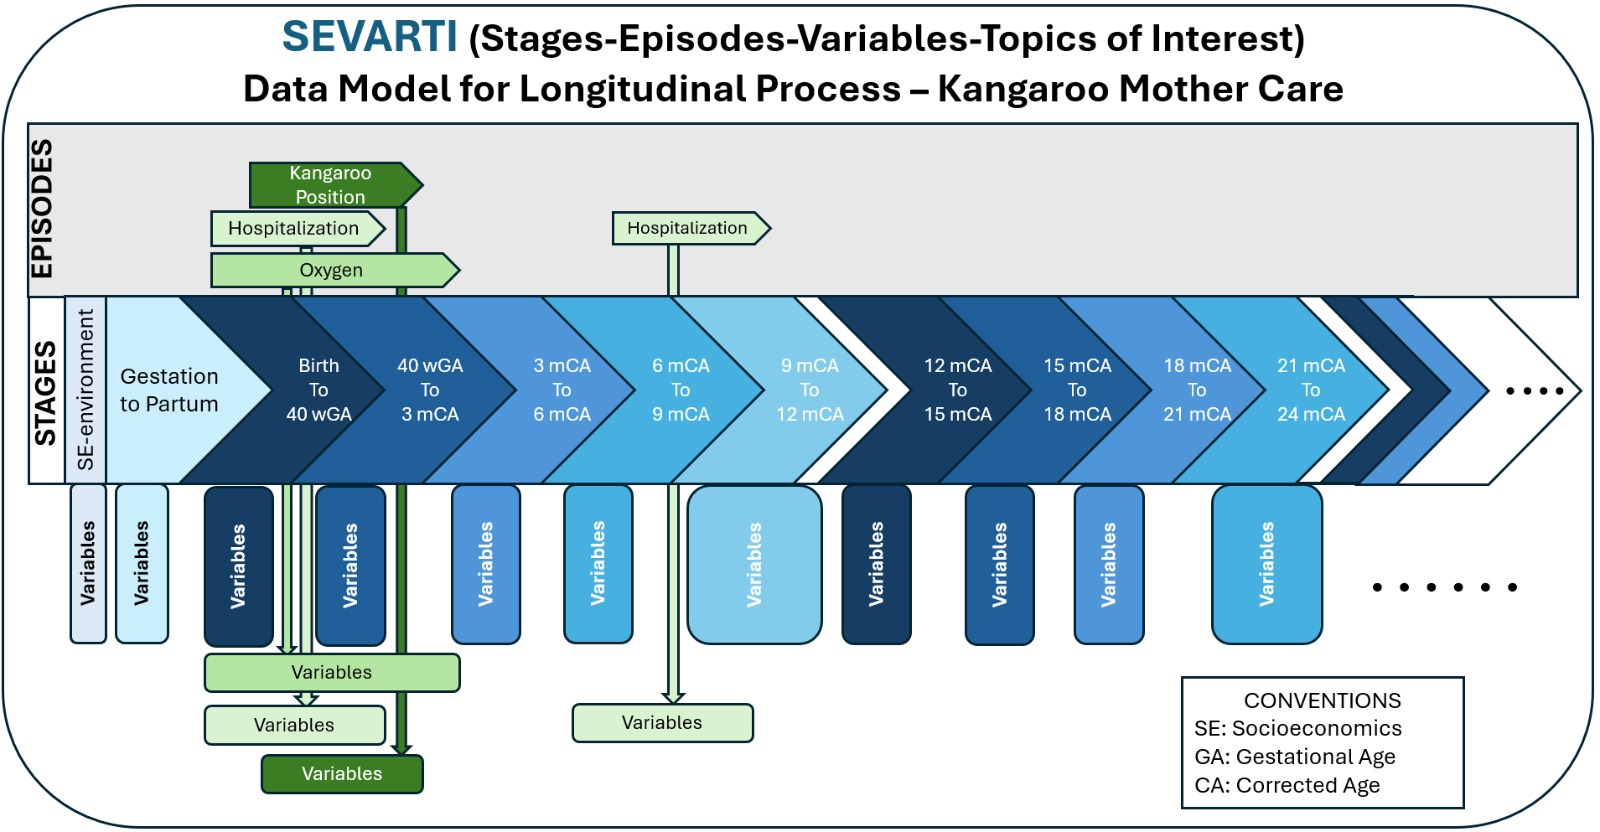
\includegraphics[width=\columnwidth]{figuras/image1.jpeg}
\caption{Modelo conceptual SEVARTI: etapas, episodios y variables vinculados al seguimiento. \fuente{Fundación Canguro, figura institucional facilitada para este estudio \cite{r4}.}}
\label{fig:1}
\end{figure}

La base original no sigue directamente la estructura SEVARTI, por eso construimos un adaptador que reúne los registros en seis entidades: esquema de variables, etapas, sujetos, mediciones, episodios y cambios conocidos en los sistemas de registro. El diccionario de variables, que pueden revisar los expertos, indica las unidades, los códigos de ausencia y las reglas de validez. Así evitamos programar reglas distintas para cada variable y podemos mantener el sistema cuando cambia la información disponible.

Para comparar las mediciones a lo largo del seguimiento usamos la edad corregida (EC), calculada a partir de la edad gestacional al nacer (EG). La Ecuación~(\ref{eq:1}) muestra el cálculo en días. Conservamos las fechas reales de las visitas, porque son necesarias para comprobar en qué momento se conocía cada dato.

\begin{equation}
\text{EC (días)} = \text{edad posnatal (días)} - 7\,(40-\text{EG})
\label{eq:1}
\end{equation}

En el corte analizado, cerca del 76 \% de las mediciones no tenía una ubicación temporal explícita. Cuando la fecha, la etapa y la edad registrada eran coherentes, el adaptador permitió reconstruir su posición en el seguimiento. Los valores faltantes se conservaron como tales y se identificaron códigos especiales, unidades incorrectas y registros incompatibles. También tuvimos en cuenta el cambio del sistema de captura ocurrido en 2022, ya que modificó patrones de registro importantes para la evaluación temporal.

Decidimos no completar automáticamente los valores faltantes ni modificar la base de origen. En lugar de ello, identificamos los registros que no debían utilizarse para aprender un valor y dejamos su ausencia explícita cuando otras estimaciones los necesitaban. Esta decisión buscó evitar que la limpieza ocultara problemas reales. La máscara de exclusión quedó versionada y afectó al 1,6 \% de 3,53 millones de datos numéricos; el 52 \% de esas exclusiones correspondió a códigos especiales.

\subsection{Etapa 1: detección y revisión de anomalías}
\label{sec:3.2}

La primera etapa de KMCPred examina cada medición desde cinco puntos de vista. Primero comprueba que su tipo, unidad y fecha sean posibles. Después busca valores inusuales, teniendo en cuenta códigos especiales y posibles errores de unidad. En el tercer nivel compara la medición con lo esperado para un niño con antecedentes similares mediante LightGBM cuantílico; el modelo no recibe como entrada el propio valor que intenta revisar. El cuarto nivel contrasta la trayectoria entre visitas y el quinto busca cambios persistentes por trimestre en residuos, datos faltantes o redondeos, utilizando CUSUM \cite{r12,r13,r14,r15,r16,r17,r25,r26}.

Para identificar valores poco habituales utilizamos medidas estadísticas robustas y tres cuantiles esperados (0,25; 0,50 y 0,75). Cuando hay suficientes datos de calibración (al menos 1/$\alpha$, es decir, 20 con el umbral $\alpha$ = 0,05 de producción), aplicamos un criterio conformal de p $\leq$ 0,05. Su objetivo es limitar las alertas sobre datos normales bajo las condiciones de calibración, aunque no garantiza que todas las alertas correspondan a errores. El sistema conserva el dato original y explica por qué debe revisarse; solo los registros claramente inconsistentes se excluyen como objetivos de aprendizaje, sin eliminar al niño completo.

Para identificar valores que se alejan considerablemente del comportamiento habitual de una variable, utilizamos una medida estadística robusta basada en la mediana y la desviación absoluta mediana (MAD). La MAD se multiplica por 1,4826 para obtener una escala comparable con la desviación estándar cuando los datos siguen aproximadamente una distribución normal \cite{r27}. Siguiendo el criterio propuesto por Iglewicz y Hoaglin \cite{r28}, consideramos potencialmente atípicos los valores cuyo puntaje z robusto supera 3,5 en valor absoluto. Esta señal no significa necesariamente que exista un error, sino que indica que la medición requiere una revisión adicional \cite{r14}.

\begin{equation}
z_{\text{rob}} = \frac{x-\operatorname{mediana}(x)}{1{,}4826\cdot \operatorname{MAD}(x)}
\label{eq:2}
\end{equation}

Además de revisar cada valor por separado, estimamos qué intervalo sería esperable según sus antecedentes y su visita. LightGBM calcula los cuantiles Q0,25, Q0,50 y Q0,75, y la Ecuación~(\ref{eq:3}) compara el valor observado con ese intervalo. La calibración conformal ayuda a decidir qué diferencias merecen revisión \cite{r15,r16,r17}.

\begin{equation}
z_{\text{ctx}} = \frac{y-Q_{0{,}50}}{(Q_{0{,}75}-Q_{0{,}25})/1{,}349}
\label{eq:3}
\end{equation}

Para detectar cambios que aparecen poco a poco, analizamos los resultados por trimestre. El método CUSUM acumula pequeñas diferencias y genera una señal cuando superan el límite establecido; en este trabajo utilizamos k = 0,5 y h = 8 \cite{r25}.

\begin{equation}
S_t = \max(0,\;S_{t-1}+r_t-k);\quad \text{alerta si } S_t>h
\label{eq:4}
\end{equation}

\subsection{Trayectorias de crecimiento}
\label{sec:3.3}

Analizamos la evolución del peso, la longitud o talla y el perímetro cefálico durante el seguimiento. Tomamos como puntos de referencia las 40 semanas de edad posmenstrual y los 3, 6, 9 y 12 meses de edad corregida. Para comparar las medidas usamos los puntajes z de los estándares OMS \cite{r29,r30}. Señalamos valores por debajo de $-$2 desviaciones estándar, descensos mayores de una desviación entre visitas y cambios que requieren revisión por su poca plausibilidad. Estas señales ayudan a orientar el seguimiento, pero no equivalen a un diagnóstico de desnutrición.

El puntaje z expresa qué tan lejos está una medición del patrón de crecimiento correspondiente a la edad y al sexo. Un valor inferior a $-$2 DE indica que la medida está por debajo del umbral de seguimiento establecido. Para calcularlo utilizamos el estándar de referencia de la OMS usando los valores L (sesgo), M (mediana) y S (coeficiente de variación), presentado en la Ecuación~(\ref{eq:5}) \cite{r29}.

\begin{equation}
z_{\text{LMS}} = \frac{(y/M)^{L}-1}{L\cdot S}
\label{eq:5}
\end{equation}

En la Ecuación~(\ref{eq:5}), y corresponde a la medida observada, mientras que L, M y S son los parámetros de la referencia OMS. Cuando L = 0 se aplica la forma logarítmica z = ln(y/M)/S. En todos los casos se conserva el indicador antropométrico y la edad correspondiente \cite{r29,r30}.

\subsection{Etapa 2: riesgos por desenlace y explicabilidad}
\label{sec:3.4}

La segunda etapa se concentra en el riesgo clínico. Entrenamos clasificadores LightGBM para cada desenlace y momento de predicción \cite{r26}, utilizando solamente la información disponible hasta la visita que se desea evaluar. Incluimos antecedentes al nacer, episodios registrados y mediciones de controles anteriores; excluimos variables que se completan más tarde para evitar que el modelo conozca información del futuro. En la exploración inicial se evaluaron 14 desenlaces. Después, junto con la revisión del alcance clínico, decidimos priorizar dos: talla baja y desarrollo psicomotor bajo a los 12 meses EC. La talla se estima en cuatro momentos (40 semanas, 3, 6 y 9 meses) y el desarrollo psicomotor a los 6 meses, para un total de cinco modelos activos o en prueba.

Separamos los niños utilizados para entrenar de los usados para probar el modelo y respetamos el orden temporal de los registros, incluyendo el cambio de captura de 2022. Después ajustamos las probabilidades mediante calibración isotónica con información más reciente del conjunto de desarrollo \cite{r18}. Para cada estimación, KMCPred puede mostrar un riesgo, su posición relativa frente al grupo de calibración y las variables con mayor contribución según TreeSHAP \cite{r21,r22,r23}. Estas contribuciones ayudan a entender el cálculo, pero no demuestran que una variable sea la causa del resultado. La decisión de emitir una alerta también depende del criterio clínico, no de un umbral universal.

Para la construcción del modelo de detección de anomalías se dividieron los datos de la siguiente manera: 40.711 niños en entrenamiento, 7.330 en calibración y 8.955 en prueba. Para el componente clínico, el conjunto de desarrollo y calibración incluyó 48.041 niños, y el de prueba, 8.955; el 15 \% de datos más reciente del conjunto de desarrollo se reservó para calibración isotónica. La separación se realizó por niño y año de nacimiento, considerando los periodos de captura anteriores y posteriores a 2022. Solo se consideraron etiquetas cuya ventana de observación ya había terminado y se retiraron variables registradas tardíamente.

\subsection{Arquitectura de aprendizaje e hiperparámetros}
\label{sec:3.5}

Las dos etapas emplean LightGBM, pero para tareas diferentes. En calidad de datos estimamos intervalos esperados mediante regresiones por cuantiles; en riesgo clínico utilizamos clasificadores binarios independientes por desenlace y visita, seguidos de calibración isotónica. La Tabla~\ref{tab:1} resume la configuración del sistema, de manera que los resultados puedan relacionarse con los parámetros utilizados \cite{r26}.

En calidad de datos utilizamos tres cuantiles y un criterio conformal de $\alpha$ = 0,05 cuando hay suficientes datos de calibración; la sección~\ref{sec:4.2} muestra cómo cambia el resultado con $\alpha$ = 0,005. En riesgo clínico entrenamos un clasificador por desenlace y visita. La Tabla~\ref{tab:1} recoge la configuración documentada. Los resultados de la exploración de 14 desenlaces y del paquete v8 pertenecen a evaluaciones diferentes.

\begin{table}[t]
\centering
\caption{Arquitectura y configuración de hiperparámetros de los modelos del pipeline}
\label{tab:1}
\footnotesize
\setlength{\tabcolsep}{2pt}
\begin{tabular}{@{}p{0.27\columnwidth}p{0.31\columnwidth}p{0.31\columnwidth}@{}}
\toprule
\textbf{Parámetro} & \textbf{Calidad: LightGBM cuantílico} & \textbf{Riesgo: LightGBM binario} \\
\midrule
Objetivo & Q0,25 / Q0,50 / Q0,75 & Clasificación por desenlace/corte \\
Tasa de aprendizaje & 0,08 & 0,05 \\
Rondas máximas & 300 & 600 \\
Parada temprana & 30 rondas & 50 rondas \\
Hojas / mínimo por hoja & 31 / 40 & 31 / 50 \\
Muestreo filas / variables & 0,8 / 0,8 & 0,8 / 0,8 \\
Máximo de bins & 63 & 63 \\
Regularización L2 & 0 (por defecto) & 1 \\
Semilla & 7 & 11 \\
Calibración & Criterio conformal; p $\leq$ 0,05 & Isotónica; 15 \% reciente \\
Casos mínimos para modelar & --- & 30 por desenlace \\
Fracción de calibración & Conjunto independiente & 15 \% más reciente (clínico) \\
\bottomrule
\end{tabular}
\end{table}

La plataforma permite ajustar varios parámetros del modelo clínico: entre 20 y 5.000 rondas, tasa de aprendizaje entre 0,005 y 0,5, de 4 a 255 hojas por árbol, de 5 a 1.000 registros por hoja y de 10 a 1.000 casos mínimos por desenlace. Sin embargo, los entrenamientos clínicos v1--v8 documentados mantuvieron 600 rondas máximas, tasa de aprendizaje de 0,05, 31 hojas y 50 registros mínimos por hoja, con parada temprana. No se realizó una búsqueda automática de hiperparámetros.

Los hiperparámetros parten de los valores por defecto de LightGBM y se ajustaron para reducir el sobreajuste, porque los modelos priorizados tienen pocos casos positivos (entre unos 110 y 510 en prueba). La tasa de aprendizaje baja de 0,1 a 0,05 para que cada árbol corrija solo una parte pequeña del error y ningún caso aislado domine el modelo; la parada temprana detiene el entrenamiento tras 50 rondas sin mejora en validación, por lo que el máximo de rondas es solo un techo. El mínimo de niños por hoja sube de 20 a 50 para que cada predicción se apoye en un grupo con suficientes casos. Cada árbol usa un 80 \% de los niños y de las variables, de modo que no dependa siempre de los mismos. La regularización L2 = 1 acerca al promedio las predicciones de las hojas con pocos niños. Se conservaron 31 hojas, porque el mínimo por hoja ya limita la complejidad de cada árbol, y se usaron 63 intervalos por variable, el valor que LightGBM recomienda para entrenar en GPU. El detector de anomalías usa valores menos restrictivos (tasa de 0,08, parada tras 30 rondas, 40 niños por hoja y L2 = 0): predice el valor esperado de cada medición, una cantidad continua y no un desenlace poco frecuente, y entrena varios modelos por variable, por lo que conviene que converja en menos rondas. La referencia usa el mismo LightGBM y los mismos hiperparámetros, solo con edad gestacional, peso al nacer y peso al ingreso, de modo que la diferencia de AUROC refleja la información añadida.

Estos parámetros permiten controlar cuánto aprende el modelo y reducir el riesgo de ajustarse demasiado a casos particulares. La tasa de aprendizaje y el número de rondas determinan cómo se construyen los árboles; las hojas y los mínimos por hoja limitan divisiones poco estables. Para facilitar la reproducción de las pruebas registramos semillas, versiones del diccionario y de los datos, particiones, número de casos positivos y artefactos utilizados.

\subsection{Protocolo de evaluación y métricas}
\label{sec:3.6}

Para evaluar la detección de anomalías trabajamos con niños distintos de los usados para entrenar e introdujimos seis tipos de errores conocidos: códigos, unidades, desviaciones de tres DE, dígitos invertidos, cambios de etapa y valores pertenecientes a otro niño. Comparamos cuántos errores detectaba KMCPred frente a las reglas de rangos, además de contar las alertas emitidas sobre registros sin perturbación. En riesgo clínico reservamos una prueba temporal independiente y comparamos la AUROC, los casos identificados dentro del 10 \% de mayor riesgo y la relación entre riesgo promedio estimado y frecuencia observada. La referencia utiliza únicamente edad gestacional, peso al nacer y peso al ingreso.

Para no depender de una sola cifra, consideramos diferentes medidas de desempeño. La AUROC permite analizar qué tan bien se distinguen los niños que presentan un desenlace de quienes no lo presentan. La precisión, sensibilidad, especificidad y F1 ayudan a entender qué ocurre cuando se establece un umbral de alerta; la matriz de confusión muestra los aciertos y errores. Cuando el desenlace es poco frecuente, también revisamos la curva precisión--recobrado (PR). Finalmente, las curvas de calibración y el puntaje de Brier permiten estudiar si el riesgo informado se parece a lo que realmente se observó \cite{r18,r24}.

Una AUROC de 0,5 indica una discriminación cercana al azar, mientras que 1 representa una separación perfecta. La curva ROC muestra la relación entre sensibilidad y falsas alarmas a distintos umbrales. La PR-AUC resulta especialmente útil cuando hay pocos casos positivos, porque ayuda a ver cuántas alertas acertadas se obtienen al identificar más casos. Ninguna de estas métricas reemplaza la revisión de la calibración, ni por sí sola demuestra utilidad clínica \cite{r18,r24}.

En las Ecuaciones~(\ref{eq:6}) y~(\ref{eq:7}) utilizamos VP, FP, FN y VN para referirnos a los verdaderos positivos, falsos positivos, falsos negativos y verdaderos negativos.

\begin{equation}
\text{Precisión}=\frac{VP}{VP+FP};\quad \text{sensibilidad}=\frac{VP}{VP+FN}
\label{eq:6}
\end{equation}

\begin{equation}
\text{Especificidad}=\frac{VN}{VN+FP};\quad F_1=\frac{2PR}{P+R}
\label{eq:7}
\end{equation}

En estas fórmulas, P significa precisión y R, sensibilidad. La exactitud se calcula como (VP+VN)/N, y el puntaje de Brier resume la diferencia entre las probabilidades estimadas y los resultados observados. Para interpretar cualquier comparación necesitamos conocer cuántos niños se evaluaron, cuántos presentaron el desenlace, qué intervalo de confianza se obtuvo y cómo se fijó el umbral antes de utilizar los datos de prueba.

\subsection{Arquitectura de servicio, trazabilidad y protección}
\label{sec:3.7}

La Figura~\ref{fig:2} resume cómo conectamos los componentes de KMCPred. Los datos se extraen de la base institucional, se organizan con SEVARTI y pasan primero por la revisión de calidad. Después se preparan los modelos de riesgo y sus versiones. Para ofrecer los resultados utilizamos FastAPI como servicio de consulta y React para las pantallas de usuario; MLflow mantiene el historial de entrenamientos y métricas. También separamos los procesos que se ejecutan con las actualizaciones semestrales de los cálculos que solicita una persona al usar la aplicación \cite{r31,r32}.

\begin{figure}[t]
\centering
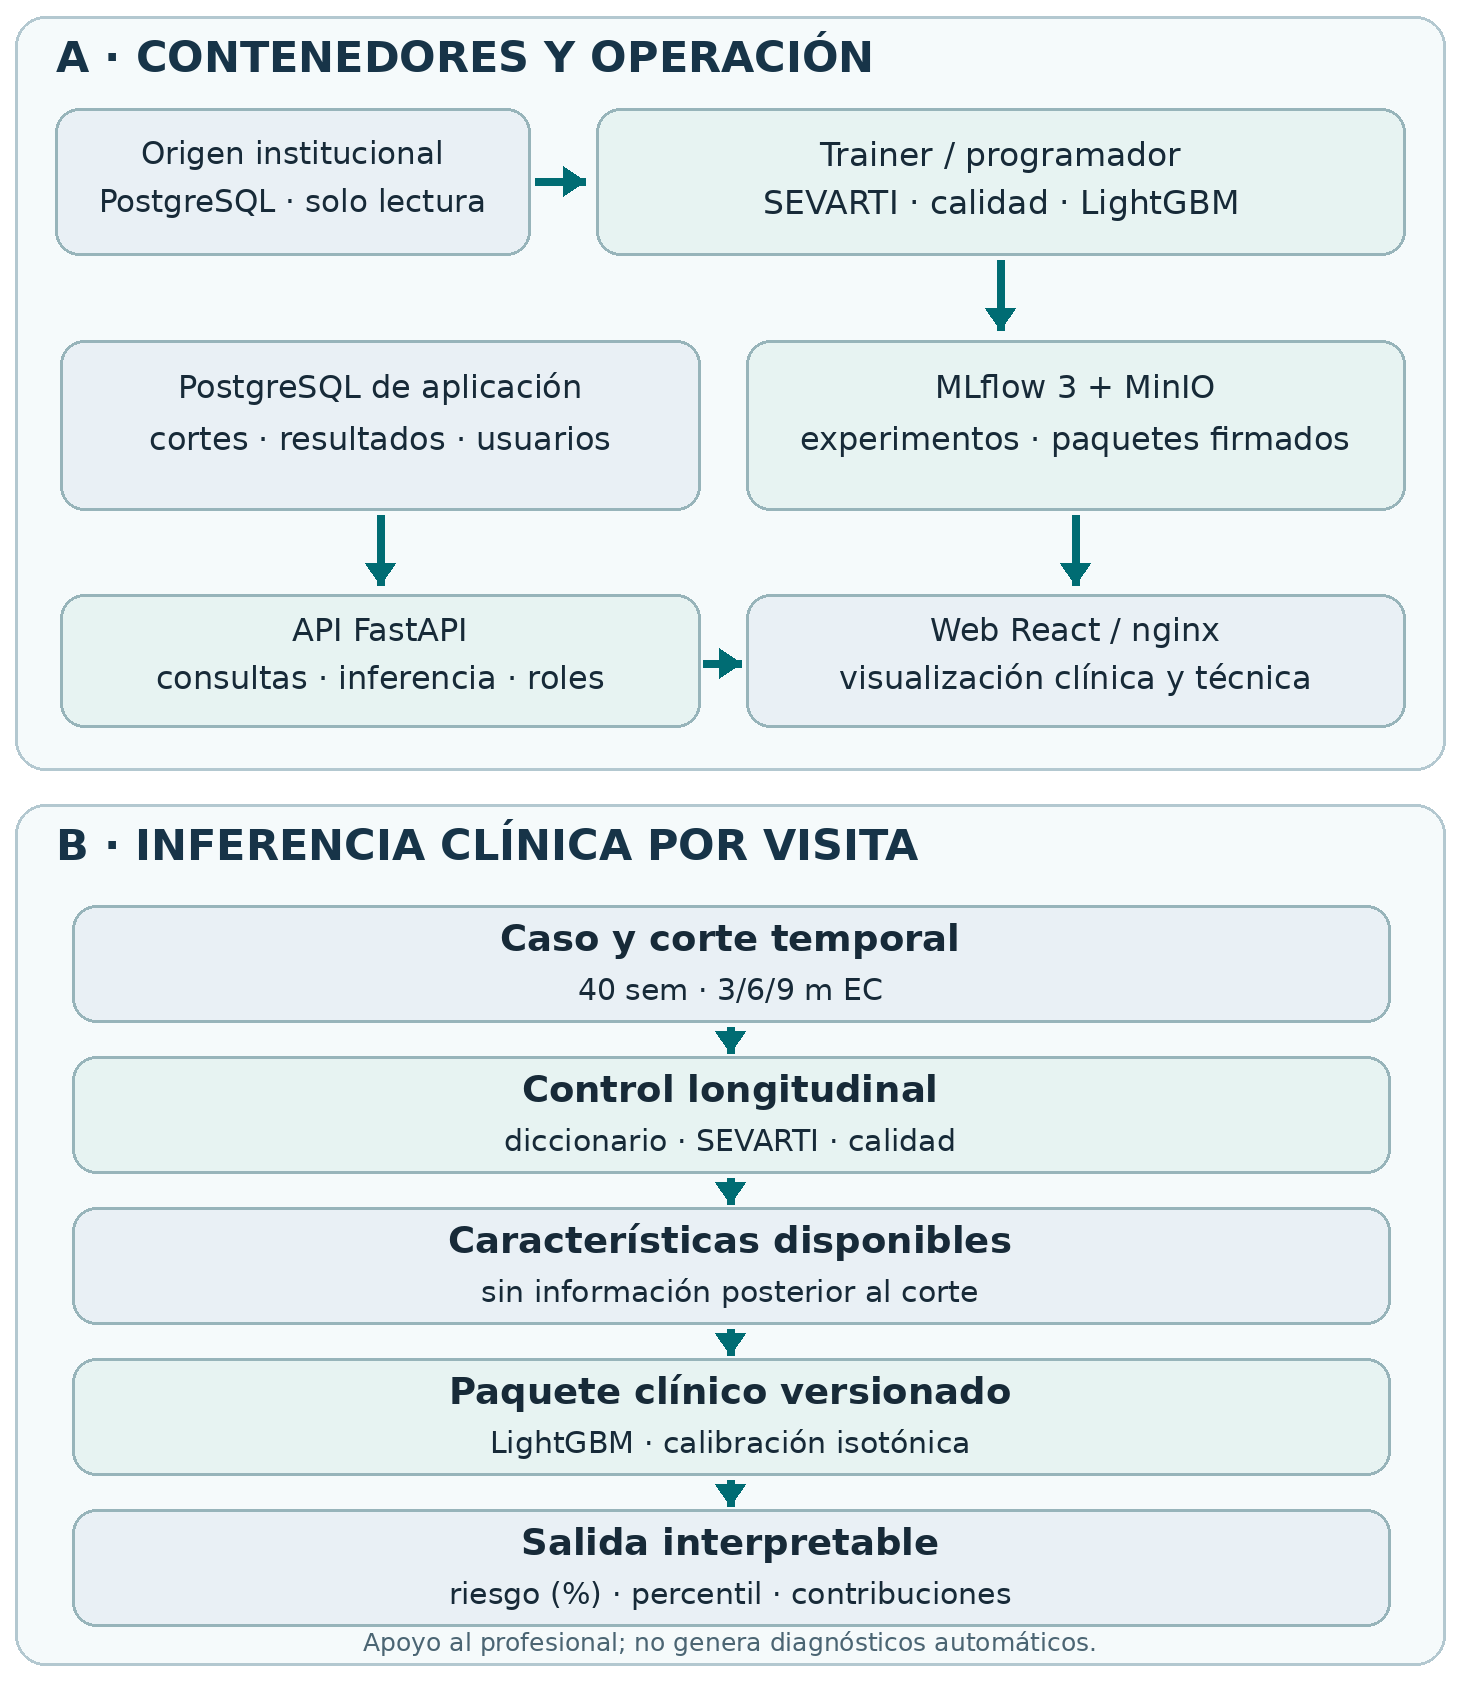
\includegraphics[width=\columnwidth]{figuras/image2.png}
\caption{Esquemas resumidos de (A) contenedores y operación y (B) inferencia por visita; elaboración propia.}
\label{fig:2}
\end{figure}

Buscamos que el profesional pueda consultar resultados sin entrar en los detalles del entrenamiento. Por eso la interfaz reúne seguimiento clínico, selección y comparación de cohortes, ficha individual y estimación de riesgo, mientras que la revisión técnica y la administración tienen apartados separados. Cada paquete conserva la versión del modelo, el diccionario y el corte de datos. En el entorno institucional se trabaja con registros autorizados; para las demostraciones se utilizan ejemplos sintéticos y permisos diferenciados.

Cuando se calcula el riesgo de un niño, la aplicación toma la información disponible hasta la visita seleccionada, prepara su trayectoria y aplica el modelo correspondiente. El resultado puede incluir el riesgo estimado, el percentil y las explicaciones disponibles. Las estimaciones de grupos grandes se ejecutan en segundo plano, y los cálculos detallados por niño no se guardan automáticamente. Esta separación busca facilitar la consulta clínica sin perder el control sobre las operaciones técnicas.

La plataforma utiliza seis servicios principales: interfaz web con React, Vite y nginx; API con FastAPI y SQLAlchemy; procesos de entrenamiento con Python y LightGBM; PostgreSQL 16; MLflow 3 para registrar modelos, y MinIO para almacenar artefactos. Los servicios se ejecutan en contenedores Docker, desplegados con Coolify sobre infraestructura propia. Además de pruebas automáticas de Python y de la web, se verifican las firmas y los archivos de los paquetes antes de utilizarlos y se aplican permisos según el rol.

\section{Resultados}
\label{sec:resultados}

\subsection{Perfil de la cohorte y calidad del registro}
\label{sec:4.1}

El corte del 24 de julio de 2026 reúne 62.043 niños y 13.884.056 mediciones. El seguimiento, sin embargo, no está completo para todos: aproximadamente el 78 \% de los niños con registro inicial llega al control de 40 semanas y el 46 \% al de 12 meses. En la revisión exploratoria encontramos 33 fechas imposibles, 985 episodios registrados antes del nacimiento y once variables cuyos rangos coincidían con los extremos observados, por lo que no resultaban útiles como control de calidad. También observamos que el redondeo del peso a 100 g pasó del 0,9 \% al 5,4 \% tras el cambio de sistema de 2022. Estos hallazgos ayudaron a definir cómo preparar y evaluar los datos.

La Figura~\ref{fig:3} muestra cómo cambia la cobertura de peso a lo largo de las visitas. Tener una medición registrada no significa necesariamente que el niño haya asistido a todos los controles. Además, cuando la información disminuye con el tiempo, los resultados obtenidos solo con los casos completos pueden dejar de representar a toda la población inicial.

\begin{figure}[t]
\centering
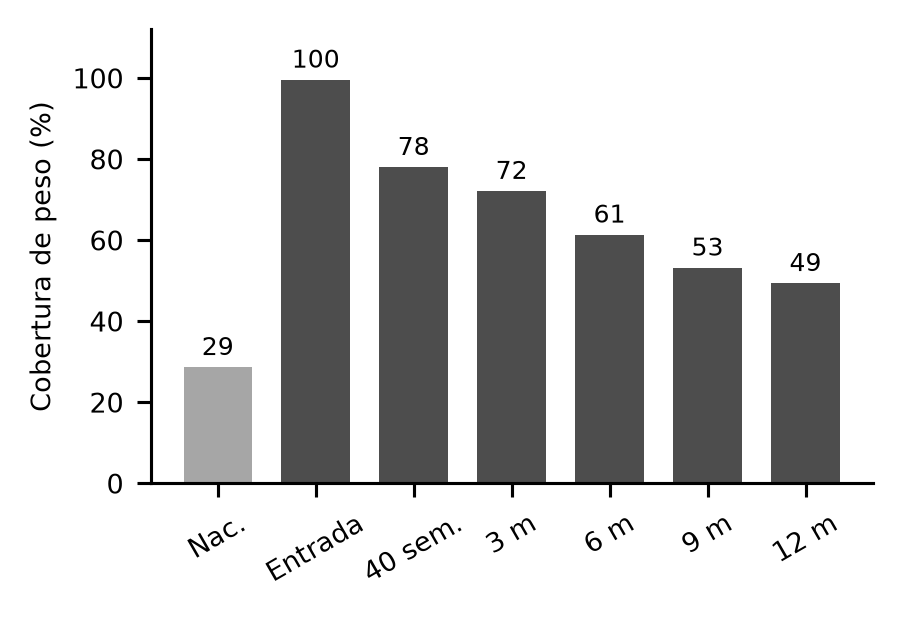
\includegraphics[width=\columnwidth]{figuras/image3.png}
\caption{Cobertura del peso por visita entre niños elegibles (corte del 24/07/2026). Elaboración propia.}
\label{fig:3}
\end{figure}

\subsection{Desempeño del detector de anomalías}
\label{sec:4.2}

Evaluamos el modelo de anomalías que está en producción (versión 7, $\alpha$ = 0,05) con los datos del corte del 24 de julio de 2026. El detector entrenó 132 modelos contextuales en 9,9 minutos. Identificó el 83,6 \% de los errores introducidos para la prueba y emitió 65,1 alertas por cada 1.000 registros limpios, frente a 14,7 de las reglas de rangos. Como muestra la Figura~\ref{fig:4}, mejoró la detección de desviaciones de tres DE (90 \% frente a 25 \%) y de etapas intercambiadas (77 \% frente a 6 \%). Los valores tomados de otro niño siguieron siendo los más difíciles de detectar (53 \%). El umbral $\alpha$ regula el equilibrio entre detectar y alertar: con $\alpha$ = 0,005, el mismo modelo detecta el 75,6 \% de los errores con 18,9 alertas por cada 1.000 registros limpios.

Estos resultados son útiles para comparar métodos, pero no representan el porcentaje de errores reales que el sistema encontraría en una clínica. Para saber cuántas alertas corresponden a problemas verdaderos hace falta la revisión de los profesionales, preferiblemente sin mostrarles previamente la predicción del modelo.

\begin{figure}[t]
\centering
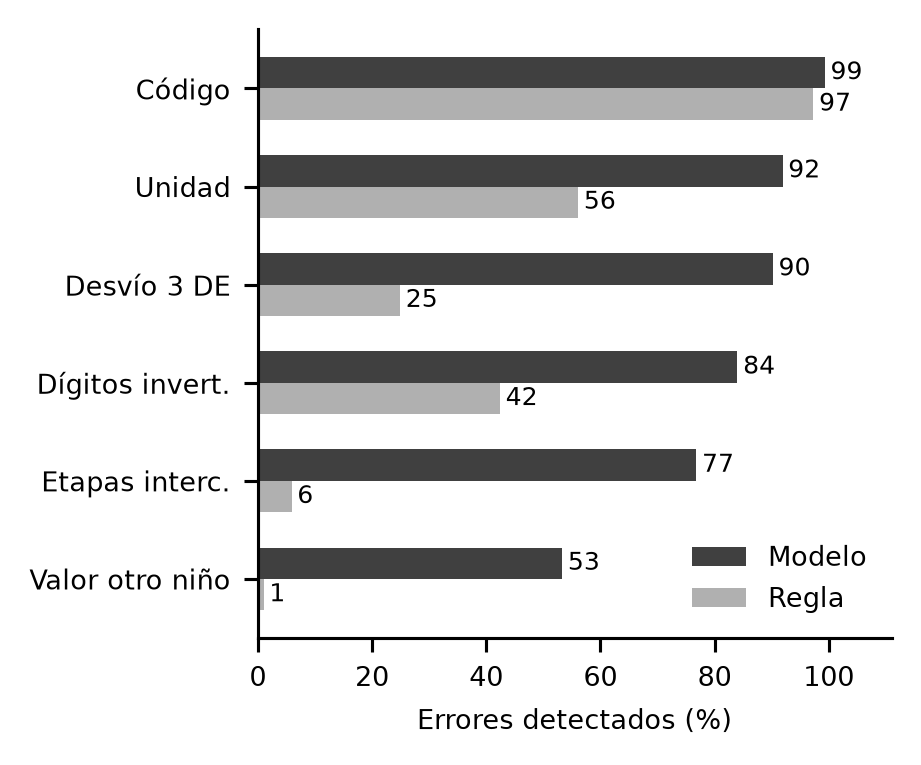
\includegraphics[width=\columnwidth]{figuras/image4.png}
\caption{Porcentaje de errores sintéticos detectados, por categoría: modelo de anomalías en producción (versión 7, $\alpha$ = 0,05) frente a la regla de rangos. Elaboración propia a partir de las métricas registradas en MLflow.}
\label{fig:4}
\end{figure}

\subsection{Evaluación retrospectiva y priorización clínica}
\label{sec:4.3}

Las particiones se describen en la sección~\ref{sec:3.4}; los N de las Tablas~\ref{tab:2} y~\ref{tab:3} son menores que la partición de prueba porque cada desenlace solo incluye a los niños con el resultado ya observado.

Al comenzar el proyecto estudiamos 14 desenlaces relacionados con readmisiones, inasistencias, uso de oxígeno y desarrollo psicomotor. Frente a una referencia sencilla, el modelo obtuvo una AUROC mayor en 13 y empató en uno (Figura~\ref{fig:5} y Tabla~\ref{tab:2}). Un resultado destacado fue la oxigenodependencia a tres meses: AUROC de 0,91 frente a 0,80. No todos los resultados fueron igualmente favorables; algunos desenlaces de inasistencia y readmisión tardía tuvieron discriminación limitada o riesgos sobreestimados.

\begin{figure}[t]
\centering
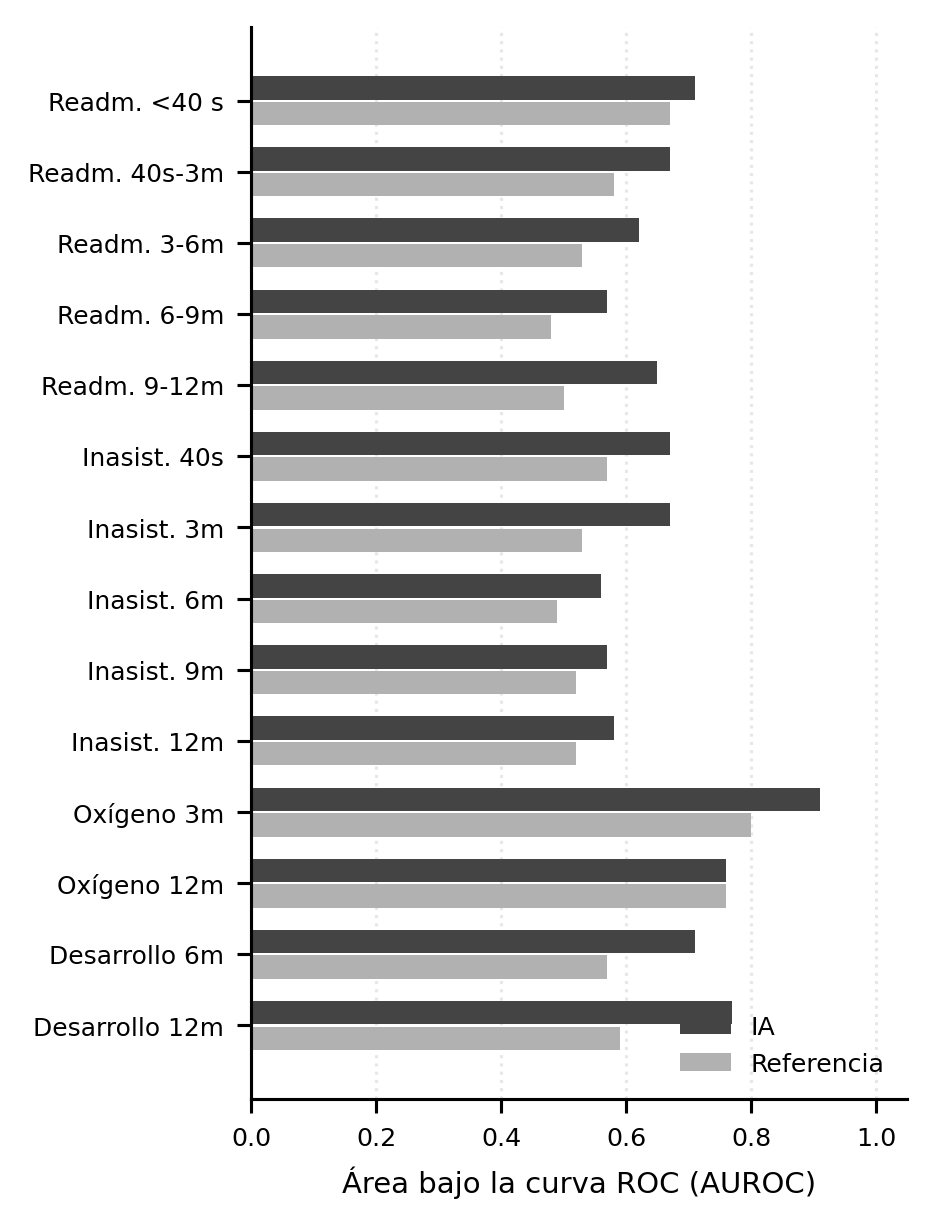
\includegraphics[width=\columnwidth]{figuras/image5.png}
\caption{Comparación de AUROC por desenlace entre el modelo completo y la referencia. Elaboración propia a partir de los resultados retrospectivos.}
\label{fig:5}
\end{figure}

La Tabla~\ref{tab:2} presenta los resultados de la evaluación inicial y el número de niños elegibles para cada desenlace. La relación R/O compara el riesgo medio estimado con la proporción observada; cuando supera 1, el modelo está sobreestimando el riesgo en promedio. Esto ocurrió, por ejemplo, en la readmisión entre 3 y 6 meses, con una relación de 2,96. Aunque el modelo distinguiera mejor a los niños que la referencia, esa diferencia nos recordó que una buena AUROC no garantiza probabilidades bien calibradas \cite{r18,r19}.

\begin{table}[t]
\centering
\caption{Discriminación y relación riesgo/observado por desenlace}
\label{tab:2}
\footnotesize
\setlength{\tabcolsep}{2pt}
\begin{tabular}{@{}lrrrr@{}}
\toprule
\textbf{Desenlace} & \textbf{N} & \textbf{AUC IA} & \textbf{AUC base} & \textbf{R/O} \\
\midrule
Readm. \textless40 s & 6.323 & 0,71 & 0,67 & 1,64 \\
Readm. 40s-3m & 3.886 & 0,67 & 0,58 & 1,39 \\
Readm. 3-6m & 3.385 & 0,62 & 0,53 & 2,96 \\
Readm. 6-9m & 2.615 & 0,57 & 0,48 & 1,59 \\
Readm. 9-12m & 2.295 & 0,65 & 0,50 & 2,01 \\
Inasist. 40s & 2.222 & 0,67 & 0,57 & 0,98 \\
Inasist. 3m & 4.338 & 0,67 & 0,53 & 0,97 \\
Inasist. 6m & 4.660 & 0,56 & 0,49 & 0,90 \\
Inasist. 9m & 3.855 & 0,57 & 0,52 & 0,84 \\
Inasist. 12m & 3.150 & 0,58 & 0,52 & 1,06 \\
Oxígeno 3m & 5.315 & 0,91 & 0,80 & 1,58 \\
Oxígeno 12m & 2.140 & 0,76 & 0,76 & 0,98 \\
Desarrollo 6m & 3.187 & 0,71 & 0,57 & 0,99 \\
Desarrollo 12m & 2.343 & 0,77 & 0,59 & 0,91 \\
\bottomrule
\end{tabular}
\end{table}

Las Figuras~\ref{fig:3}--\ref{fig:5} se elaboraron con los resultados de la evaluación retrospectiva descrita; son gráficas de síntesis preparadas por el equipo.

A partir de las observaciones del experto clínico, decidimos centrar KMCPred en dos desenlaces a los 12 meses EC: talla baja y desarrollo psicomotor bajo. El paquete clínico v8 del 21 de noviembre de 2026 incluye cuatro modelos de talla baja, que hacen estimaciones desde las 40 semanas de edad posmenstrual y los 3, 6 y 9 meses EC, y uno de desarrollo psicomotor, calculado a los 6 meses EC, ver figura~\ref{fig:6}.

\begin{figure}[t]
\centering
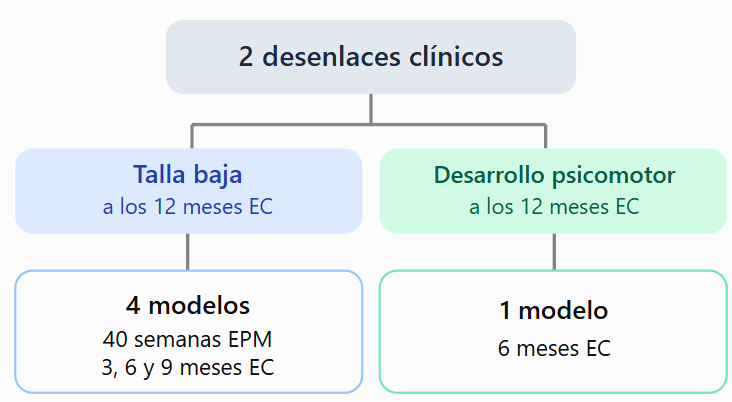
\includegraphics[width=\columnwidth]{figuras/image6.png}
\caption{Relación de modelos y desenlaces abordados. \fuente{Elaboración propia}}
\label{fig:6}
\end{figure}

La Tabla~\ref{tab:3} reúne sus resultados en una evaluación temporal independiente. No mezclamos esas cifras con los 14 desenlaces de la exploración inicial; por eso la referencia de desarrollo psicomotor es 0,59 en la Tabla~\ref{tab:2} y 0,62 en la Tabla~\ref{tab:3}: la primera proviene de la exploración inicial y la segunda, del entrenamiento n.º 15. Además, la categoría «desarrollo psicomotor bajo» se definió para este proyecto y no debe entenderse como diagnóstico clínico.

\begin{table}[t]
\centering
\caption{Resultados de los cinco modelos predictivos asociados a los dos desenlaces clínicos priorizados}
\label{tab:3}
\footnotesize
\setlength{\tabcolsep}{2pt}
\begin{tabular}{@{}p{0.24\columnwidth}p{0.19\columnwidth}p{0.22\columnwidth}p{0.12\columnwidth}p{0.15\columnwidth}@{}}
\toprule
\textbf{Desenlace y corte} & \textbf{N (prev.)} & \textbf{AUROC IA (IC 95\%)} & \textbf{AUROC base} & \textbf{PR-AUC / F1} \\
\midrule
Psicomotor 12m · 6m & 2.343 (4,7\%) & 0,77 (0,72-0,81) & 0,62 & 0,21 / 0,27 \\
Talla baja 12m · 40s & 2.072 (17,6\%) & 0,79 (0,77-0,81) & 0,61 & 0,43 / 0,38 \\
Talla baja 12m · 3m & 2.625 (19,4\%) & 0,86 (0,84-0,87) & 0,60 & 0,61 / 0,46 \\
Talla baja 12m · 6m & 2.420 (19,1\%) & 0,91 (0,89-0,92) & 0,59 & 0,74 / 0,57 \\
Talla baja 12m · 9m & 2.210 (18,9\%) & 0,93 (0,92-0,94) & 0,60 & 0,80 / 0,61 \\
\bottomrule
\end{tabular}
\end{table}

En talla baja encontramos que el desempeño mejora a medida que se dispone de más controles: la AUROC pasó de 0,79 a las 40 semanas a 0,93 a los 9 meses. No obstante, una predicción a los 9 meses deja menos tiempo para actuar que una realizada desde el primer control. A los 6 meses, el modelo alcanzó PR-AUC de 0,74 y F1 de 0,57 para el 10 \% de mayor riesgo; su riesgo promedio estimado (19,5 \%) fue cercano a la frecuencia observada (19,1 \%). Para desarrollo psicomotor, con una prevalencia de 4,7 \%, se obtuvo AUROC de 0,77, precisión de 19,7 \% y F1 de 0,27. Estas cifras muestran potencial, pero también la necesidad de estudiar cuántas alertas podría revisar el equipo clínico.

Al alertar al 10 \% de mayor riesgo, el modelo de talla baja de los 6 meses obtuvo sensibilidad de 43,2 \%, precisión de 82,2 \% y F1 de 0,57. Con información de las 40 semanas, las cifras fueron 29,9 \%, 52,7 \% y 0,38. La comparación ilustra una decisión importante: con más información podemos ganar precisión, pero perdemos parte de la anticipación. Las subcohortes evaluadas tampoco son idénticas, de modo que estas diferencias no demuestran por sí solas un beneficio clínico.

\subsubsection{Matriz de confusión y costos de alertar}
\label{sec:4.3.1}

Como ejemplo del efecto de los umbrales, retomamos el experimento inicial de oxigenodependencia a tres meses. De 5.315 niños, 201 presentaron el desenlace (3,8 \%). Al alertar al 10 \% de mayor riesgo se obtuvieron 143 verdaderos positivos, 389 falsos positivos, 58 falsos negativos y 4.725 verdaderos negativos (Figura~\ref{fig:7}).

\begin{figure}[t]
\centering
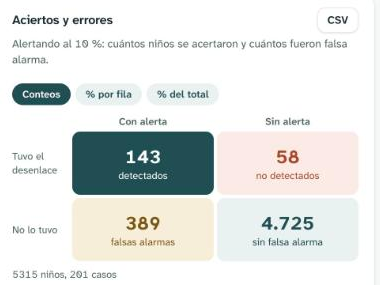
\includegraphics[width=\columnwidth]{figuras/image7.png}
\caption{Matriz de confusión de oxigenodependencia a tres meses al alertar al 10 \% con mayor riesgo (evaluación anterior al paquete clínico v8).}
\label{fig:7}
\end{figure}

Cuando aumentamos la proporción de niños alertados del 5 \% al 20 \%, la sensibilidad pasó del 47,3 \% al 88,1 \%, pero la precisión bajó del 35,7 \% al 16,7 \% (Tabla~\ref{tab:4}). Esto muestra por qué la decisión sobre el umbral debe tomarse con los profesionales: detectar más casos también implica revisar más alertas que finalmente no tendrán el desenlace.

\begin{table}[t]
\centering
\caption{Métricas de oxigenodependencia a tres meses según la proporción alertada (evaluación histórica)}
\label{tab:4}
\footnotesize
\setlength{\tabcolsep}{2pt}
\begin{tabular}{@{}lrrrr@{}}
\toprule
\textbf{Proporción} & \textbf{Sensibilidad} & \textbf{Especificidad} & \textbf{Precisión} & \textbf{F1} \\
\midrule
5 \% & 47,3 \% & 96,7 \% & 35,7 \% & 0,41 \\
10 \% & 71,1 \% & 92,4 \% & 26,9 \% & 0,39 \\
20 \% & 88,1 \% & 82,7 \% & 16,7 \% & 0,28 \\
\bottomrule
\end{tabular}
\end{table}

La Figura~\ref{fig:8} presenta las curvas ROC y precisión--recobrado del modelo de talla baja a los 12 meses EC, utilizando información hasta los 6 meses EC. Su AUROC de 0,91 y PR-AUC de 0,74 reflejan una buena capacidad para diferenciar los casos en la prueba temporal. Aun así, estas curvas no indican por sí solas si el porcentaje de riesgo es acertado; para eso revisamos también la calibración de la Figura~\ref{fig:10}.

\begin{figure}[t]
\centering
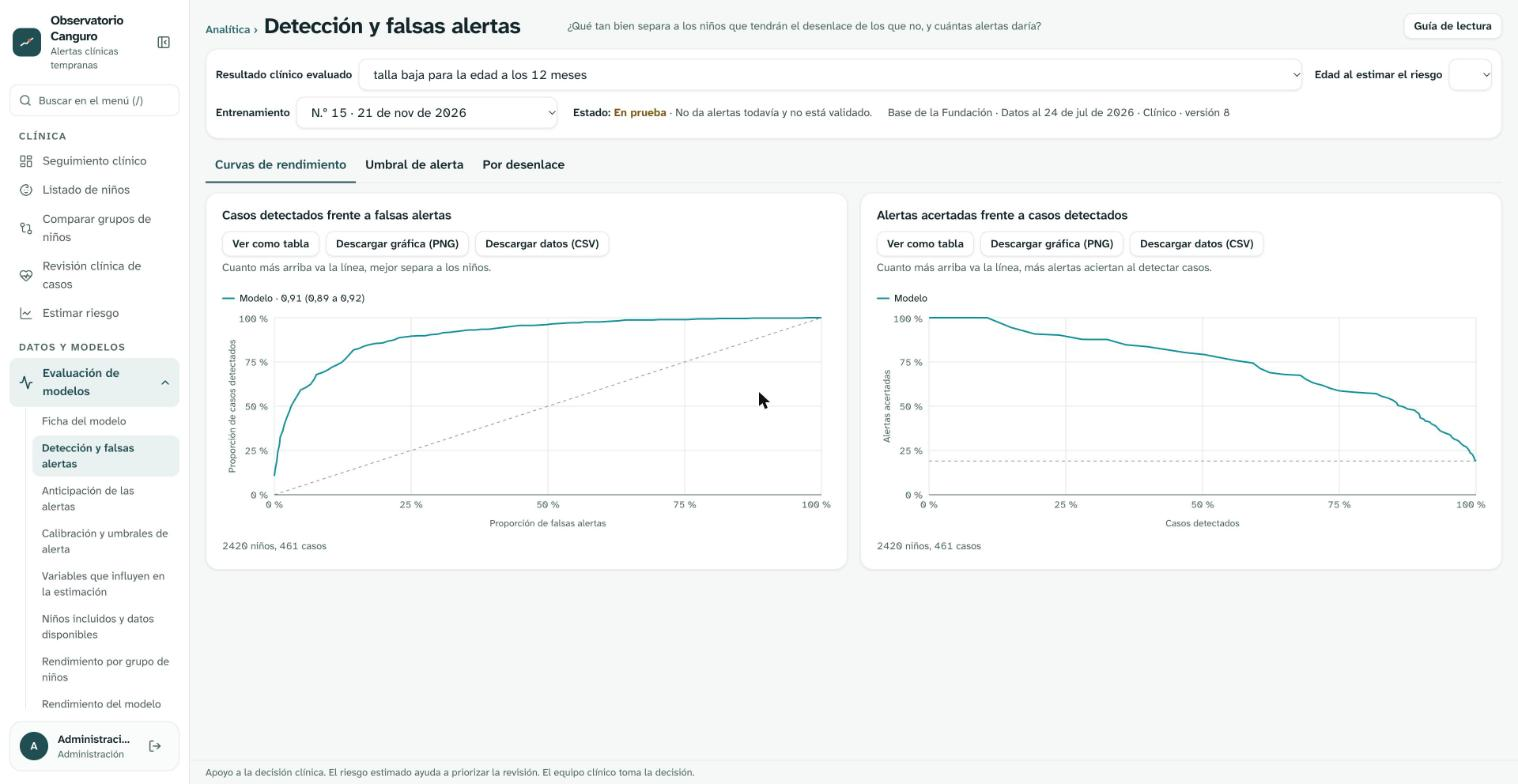
\includegraphics[width=\columnwidth]{figuras/image8.jpg}
\caption{Curvas ROC y precisión--recobrado para talla baja a los 12 meses, estimada a los 6 meses EC}
\label{fig:8}
\end{figure}

\subsection{Crecimiento, denominadores y anticipación}
\label{sec:4.4}

Según los estándares OMS, la proporción de registros por debajo de $-$2 DE fue mayor para talla (18,6--22,4 \%, según la visita) que para peso (10,6--12,0 \%). La Tabla~\ref{tab:5} resume esos resultados iniciales por medición. En la aplicación actual revisamos también el número de niños, para evitar contar varias veces a quienes tienen más de un dato: a las 40 semanas había 24.007 registros de peso, pero correspondían a 20.800 niños. Esta distinción es importante para interpretar cualquier porcentaje clínico.

\begin{table}[t]
\centering
\caption{Porcentaje de registros antropométricos con z inferior a $-$2 DE en el análisis inicial (el recuento por niño de la versión publicada es distinto)}
\label{tab:5}
\footnotesize
\setlength{\tabcolsep}{2pt}
\begin{tabular}{@{}lrrrrr@{}}
\toprule
\textbf{Indicador} & \textbf{40 sem.} & \textbf{3 m} & \textbf{6 m} & \textbf{9 m} & \textbf{12 m} \\
\midrule
Peso & 11,7 & 10,6 & 12,0 & 11,5 & 10,7 \\
Talla & 20,5 & 22,4 & 20,4 & 18,9 & 18,6 \\
P. cefálico & 1,1 & 4,2 & 3,3 & 3,3 & 3,7 \\
\bottomrule
\end{tabular}
\end{table}

\fuente{análisis antropométrico inicial del corte}. Los porcentajes por registro no equivalen necesariamente a prevalencias por niño; la versión publicada corrigió la agregación. Una señal de z \textless{} $-$2 es motivo de vigilancia, no diagnóstico automático.

\subsection{Aplicación, trazabilidad y evidencia operativa}
\label{sec:4.5}

KMCPred se encuentra disponible en \url{https://maia.canbby.com}. Su recorrido permite consultar el seguimiento clínico, explorar grupos mediante filtros, comparar dos cohortes, revisar la ficha de un niño y estimar riesgos. Los apartados técnicos incluyen evaluación de modelos y operación del sistema (Tabla~\ref{tab:6}). La información a la que accede cada persona depende de su perfil: Consulta, Experto clínico, Experto en datos o Administración.

\begin{table}[t]
\centering
\caption{Recorrido funcional de la aplicación}
\label{tab:6}
\footnotesize
\setlength{\tabcolsep}{2pt}
\begin{tabular}{@{}p{0.34\columnwidth}p{0.58\columnwidth}@{}}
\toprule
\textbf{Módulo} & \textbf{Composición} \\
\midrule
Seguimiento clínico & Cohorte, filtros, crecimiento y resultados a 12 m \\
Comparar grupos & Cohortes A/B con criterios, tamaño y gráficos \\
Predicción individual & Caso sintético por visita, riesgo y versión (Fig.~\ref{fig:12}) \\
Evaluación de modelos & Ficha, ROC/PR, calibración e interpretabilidad (Figs.~\ref{fig:8}--\ref{fig:11}) \\
Calidad y operación & Alertas, revisión, administración y configuración \\
\bottomrule
\end{tabular}
\end{table}

La Tabla~\ref{tab:7} muestra los conteos de las matrices de confusión de los cinco modelos del paquete v8 cuando se alerta al 10 \% de mayor riesgo. Son los valores con que se calcularon el F1 de la Tabla~\ref{tab:3} y la sensibilidad y precisión citadas en la sección~\ref{sec:4.3}.

\begin{table}[t]
\centering
\caption{Matrices de confusión de los cinco modelos del paquete v8 al alertar al 10 \% de mayor riesgo (prueba temporal, entrenamiento n.º 15)}
\label{tab:7}
\footnotesize
\setlength{\tabcolsep}{2pt}
\begin{tabular}{@{}lrrrr@{}}
\toprule
\textbf{Modelo · corte} & \textbf{VP} & \textbf{FP} & \textbf{FN} & \textbf{VN} \\
\midrule
Psicomotor 12 m · 6 m EC & 46 & 188 & 63 & 2.046 \\
Talla baja 12 m · 40 sem. & 109 & 98 & 256 & 1.609 \\
Talla baja 12 m · 3 m EC & 179 & 83 & 331 & 2.032 \\
Talla baja 12 m · 6 m EC & 199 & 43 & 262 & 1.916 \\
Talla baja 12 m · 9 m EC & 196 & 25 & 221 & 1.768 \\
\bottomrule
\end{tabular}
\end{table}

El servidor utilizado dispone de un procesador AMD Ryzen 9 7900X, una GPU RTX 5060 Ti y 30,45 GiB de RAM. En 17 predicciones individuales realizadas desde el navegador el 21 de noviembre de 2026, el tiempo mediano fue 2,54 s y el percentil 95 alcanzó 2,61 s. Entrenar los cinco modelos clínicos v8 tomó aproximadamente tres minutos. Son resultados de esas pruebas puntuales; no permiten afirmar cómo respondería el sistema con muchos usuarios simultáneos.

La Figura~\ref{fig:9} recoge la ficha del modelo de talla baja a los 12 meses, estimada a los 6 meses EC. En la plataforma este modelo aparece «En prueba», por lo que sus resultados deben entenderse como parte de la evaluación y no como una herramienta clínica ya validada. Al comparar grupos A/B, también es importante mostrar claramente los filtros utilizados, los tamaños de ambos grupos y los datos disponibles.

\begin{figure}[t]
\centering
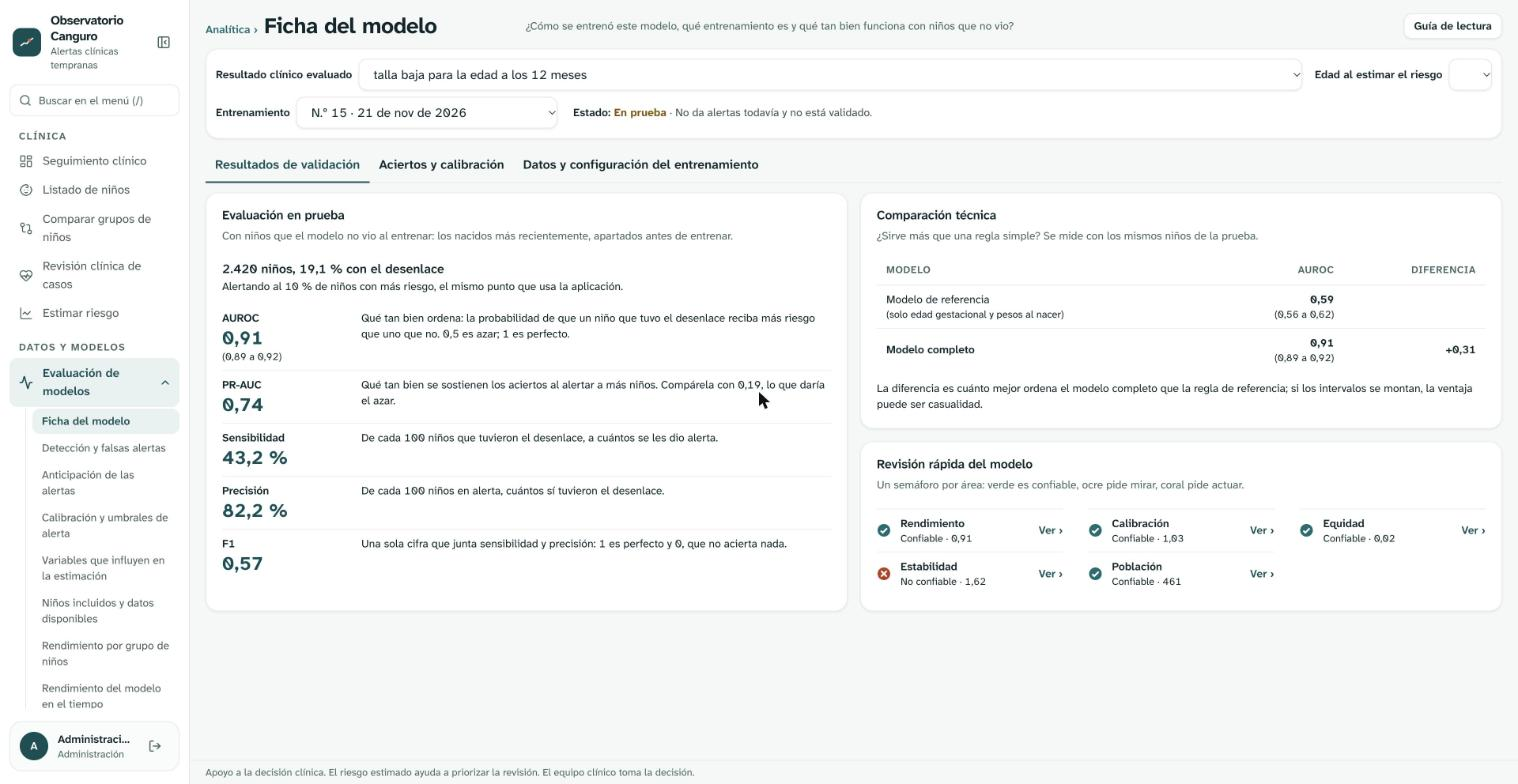
\includegraphics[width=\columnwidth]{figuras/image9.jpg}
\caption{Ficha del modelo: talla baja a 12 meses estimada a 6 meses EC, entrenamiento n.º 15 y paquete v8.}
\label{fig:9}
\end{figure}

La Figura~\ref{fig:10} compara, por grupos de riesgo, las probabilidades calculadas para talla baja a los 12 meses desde los 6 meses EC con los resultados observados. El promedio predicho fue 19,5 \% y el observado 19,1 \% (relación 1,03; error medio de calibración 0,026; Brier 0,087). Es una señal favorable dentro de esta evaluación retrospectiva, pero no reemplaza la validación prospectiva ni garantiza que el modelo funcione igual en todos los subgrupos.

\begin{figure}[t]
\centering
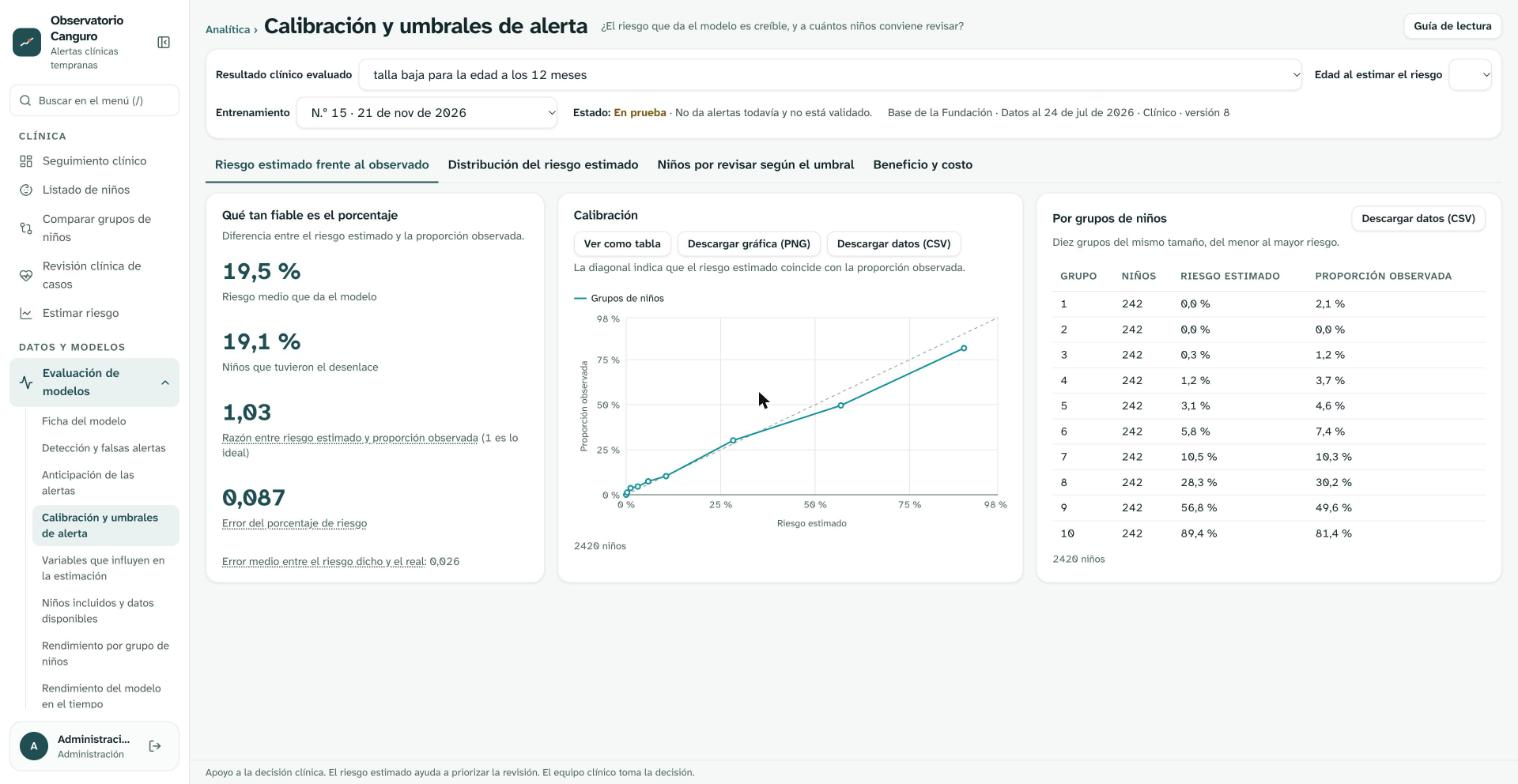
\includegraphics[width=\columnwidth]{figuras/image10.jpg}
\caption{Calibración por deciles de la probabilidad de talla baja a 12 meses calculada a los 6 meses EC (paquete v8).}
\label{fig:10}
\end{figure}

La Figura~\ref{fig:11} presenta las variables con mayor importancia global en el modelo de desarrollo psicomotor bajo, medida como la ganancia que aporta cada variable en LightGBM. Estas importancias muestran patrones aprendidos, no causas clínicas. TreeSHAP se usa en la explicación individual de cada niño. Algunas variables aparecen con su código del diccionario del Observatorio Canguro, tal como las muestra la plataforma.

\begin{figure}[t]
\centering
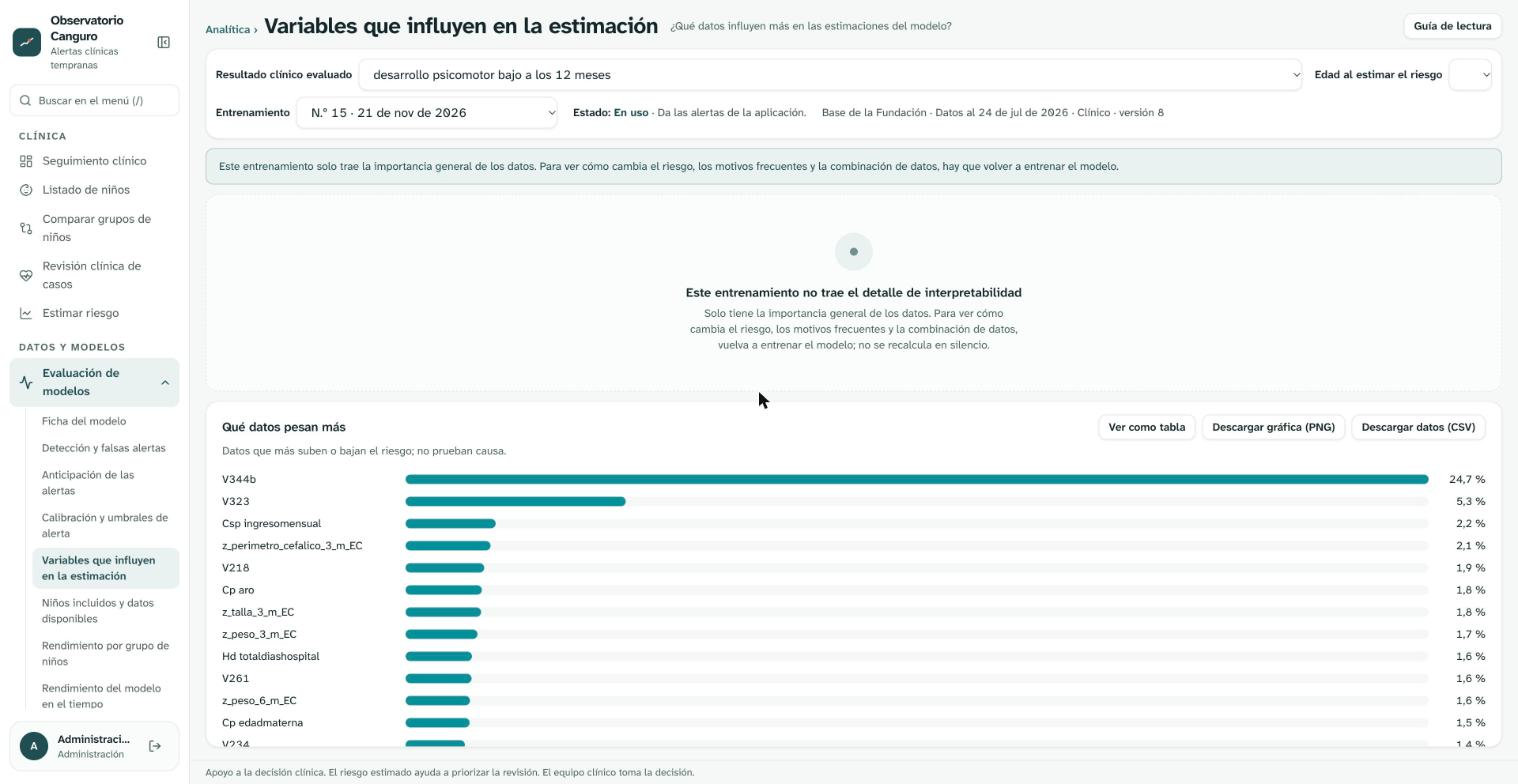
\includegraphics[width=\columnwidth]{figuras/image11.jpg}
\caption{Importancia global de variables (ganancia de LightGBM) del desenlace desarrollo psicomotor bajo a los 12 meses; captura del paquete activo. Las variables se muestran con su código del diccionario.}
\label{fig:11}
\end{figure}

La Figura~\ref{fig:12} presenta un niño simulado cuyo riesgo de talla baja a los 12 meses se consulta desde las 40 semanas y los 3, 6 y 9 meses EC; cada estimación debe usar solo datos disponibles hasta su corte.

\begin{figure}[t]
\centering
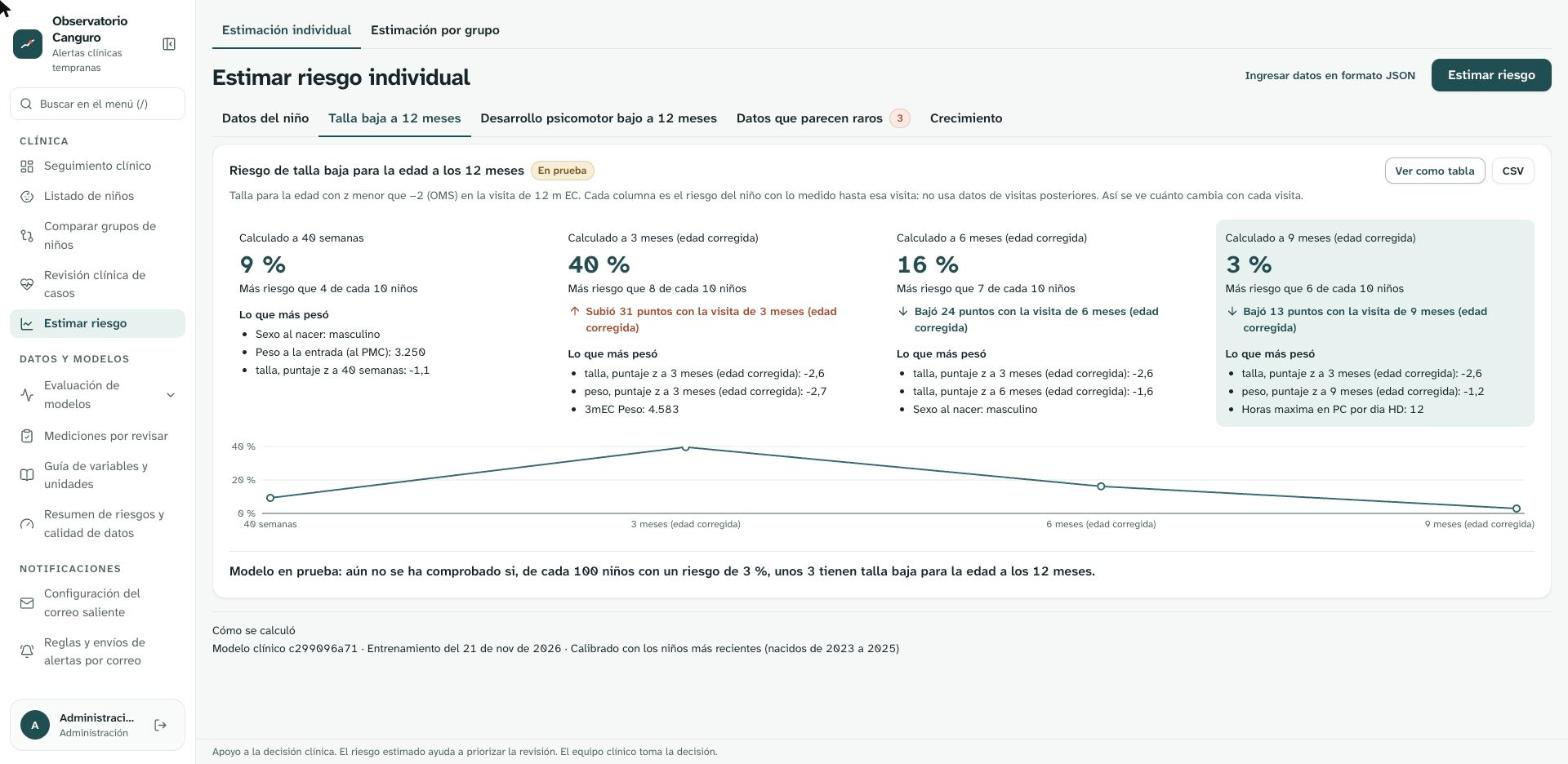
\includegraphics[width=\columnwidth]{figuras/image12.jpg}
\caption{Estimación de talla baja a 12 meses para un niño simulado desde distintas visitas; cada cálculo usa solo información previa a su corte.}
\label{fig:12}
\end{figure}

\section{Discusión}
\label{sec:discusion}

\subsection{Interpretación clínica y contraste con trabajos relacionados}
\label{sec:5.1}

Los trabajos revisados sobre crecimiento en programas canguro \cite{r5,r7} nos llevaron a prestar atención a la trayectoria entre visitas, en lugar de depender de una sola medida. Los estudios sobre neurodesarrollo \cite{r8,r9,r10} también respaldan el uso de información temprana, aunque no permiten comparar directamente sus resultados con los nuestros. Lo que consideramos más valioso de KMCPred es haber reunido la revisión del dato, la predicción por visita y la consulta de resultados en una misma herramienta.

\subsection{Arquitectura, pruebas y reproducibilidad}
\label{sec:5.2}

Para que otra persona pueda reproducir un resultado, necesitamos saber qué datos, versión del diccionario, modelo y parámetros se utilizaron. KMCPred conserva esa información mediante MLflow, los paquetes de modelos y sus registros de ejecución (Figura~\ref{fig:2}). Además, superó 534 pruebas de la aplicación web distribuidas en 48 archivos y 783 pruebas de Python; una prueba quedó omitida. Esto respalda el funcionamiento técnico revisado, pero no equivale a una evaluación clínica con pacientes.

En la operación habitual, el sistema lee la base institucional, organiza los datos, identifica registros dudosos, entrena y calibra modelos y registra los resultados. El paquete se aprueba antes de calcular de nuevo los riesgos. Los procesos programados siguen el calendario semestral de actualización de la fuente. Se documentaron cuatro corridas completas sobre los 62.043 niños, aunque todavía no contamos con una prueba que mida el comportamiento con varios usuarios simultáneos.

Las pruebas disponibles muestran que es posible navegar por la plataforma y utilizar sus funciones principales.

\subsection{Evaluación económica y sostenibilidad}
\label{sec:5.3}

Estimamos el coste de desarrollo de KMCPred en 48.485.707 COP para 16 semanas de trabajo. La mayor parte corresponde al tiempo del equipo (40 millones; 82,5 \%), seguido de infraestructura (3,02 millones), software (1,06 millones) e imprevistos (4,41 millones). De ese total, 2,53 millones (5,2 \%) se clasificaron como aportes en efectivo y el resto se valoró como trabajo o recursos en especie. El uso de software abierto y de un servidor propio permite evitar pagos por cada predicción, pero no significa que operar la plataforma sea gratuito. El presupuesto incluye una máquina virtual en la nube como referencia; el coste real de mantener el despliegue en Coolify no se ha medido.

\subsection{Limitaciones, equidad y validez clínica}
\label{sec:5.4}

El proyecto tiene limitaciones que deben ser consideradas, entre ellas que solo el 46 \% de los niños con registro inicial llega al control de 12 meses, y el cambio de sistema en 2022 puede afectar la comparación entre periodos. También necesitamos entender mejor cómo varía el desempeño entre grupos de niños y con el paso del tiempo. Aunque se exportaron indicadores de estabilidad y equidad, los archivos no identifican con suficiente detalle el modelo y la corrida; algunas series contienen entre 21 y 45 niños por trimestre y ciertos subgrupos apenas cuatro.

Las explicaciones de TreeSHAP describen asociaciones que el modelo encontró en los datos; no prueban causas. Por eso, ningún porcentaje de riesgo debe utilizarse por sí solo para decidir tratamientos o remisiones. Los registros institucionales se mantienen bajo acceso controlado y los ejemplos públicos son sintéticos. Aún necesitamos completar la revisión ciega por profesionales y, más adelante, una validación prospectiva que permita valorar el sistema en condiciones de uso real.

\section{Conclusiones y trabajo futuro}
\label{sec:conclusiones}

\begin{itemize}
\item KMCPred integra verificación longitudinal de calidad y predicción interpretable por visita sobre una cohorte institucional extensa. La evaluación del modelo de anomalías en producción encontró 83,6 \% de detección de perturbaciones sintéticas con 65,1 alertas/1.000 datos limpios, y la exploración inicial mostró mejoras de AUROC en 13/14 desenlaces frente a una referencia reducida. En la versión publicada se priorizaron cinco modelos clínicos para dos familias de desenlaces a 12 meses: talla baja (AUROC 0,79--0,93) y desarrollo psicomotor bajo (0,77). Estos resultados reflejan validación retrospectiva y no deben trasladarse como rendimiento prospectivo garantizado.
\item Uno de los aprendizajes del proyecto fue que un modelo no basta si el personal no puede entender qué datos analiza o de dónde sale un resultado. Por eso dedicamos parte del desarrollo a organizar los registros con SEVARTI, identificar las visitas disponibles, mostrar las cohortes y separar las funciones clínicas de las técnicas. También fue importante corregir el recuento por niño y advertir cuando una predicción corresponde a una selección anterior. Las gráficas deben leerse siempre junto con el número de niños evaluados, la fecha del corte y el estado del modelo.
\item Como trabajo futuro proponemos empezar por una revisión ciega con especialistas y una evaluación prospectiva sin influir en las decisiones de atención. También necesitamos comprobar el desempeño en otras poblaciones y subgrupos, vigilar los cambios temporales y recalibrar los modelos cuando sea necesario. Quedan pendientes las pruebas de usabilidad, la evaluación de varios usuarios simultáneos y la comparación con reglas clínicas sencillas, como la última talla disponible. Además, sería importante incorporar curvas de crecimiento específicas para niños prematuros antes de las 40 semanas de edad posmenstrual, tomando como referencia los trabajos de Fenton y Kim \cite{r33} y los estándares INTERGROWTH-21st \cite{r34}. Finalmente, los umbrales de alerta deberían acordarse con la Fundación Canguro, teniendo en cuenta tanto los casos identificados como el esfuerzo de revisión que implican.
\end{itemize}


\section*{Agradecimientos}
Se agradece a la Fundación Canguro y al profesor José Tiberio Hernández por el acompañamiento académico y la documentación institucional utilizada en este proyecto.

\section*{Declaración de uso de IA generativa y contribución de autoría}
Para la revisión de la redacción de este documento y búsqueda de información de estado del arte se utilizaron ChatGPT y Claude como herramientas de apoyo. No se generaron datos ni se sustituyeron experimentos o decisiones del equipo, todo el contenido fue revisado y validado por los autores.

% Bibliografía IEEE en orden de primera cita (orden de primera cita (IEEE)).
\begin{thebibliography}{34}
\bibitem{r1}
World Health Organization, \emph{WHO Recommendations for Care of the Preterm or Low-Birth-Weight Infant}. Geneva: WHO, 2022.

\bibitem{r2}
N. Charpak, R. Tessier, J. G. Ruiz et al., ``Twenty-year follow-up of kangaroo mother care versus traditional care,'' \emph{Pediatrics}, vol. 139, no. 1, e20162063, 2017.

\bibitem{r3}
N. Charpak and A. Montealegre-Pomar, ``Follow-up of Kangaroo Mother Care programmes in the last 28 years: results from a cohort of 57\,154 low-birth-weight infants in Colombia,'' \emph{BMJ Global Health}, vol. 8, no. 5, 2023.

\bibitem{r4}
Fundación Canguro, ``Modelo conceptual SEVARTI y diccionario de variables del Observatorio Canguro,'' especificación y material gráfico institucional proporcionados para este estudio, 2026 (material técnico no publicado).

\bibitem{r5}
S. E. Melo, O. O. Melo, and N. Suarez, ``Modelo multinivel de tasa global de ganancia de peso en el programa madre canguro en Bogotá,'' \emph{Revista de Salud Pública}, vol. 18, no. 2, pp. 238--250, 2016, doi: 10.15446/rsap.v18n2.44661.

\bibitem{r6}
Z. Ren, W. Gao, Q. Wang et al., ``Predictive role of NICU-related stress, postpartum depression trajectory and family coping on growth trajectory of moderate-to-late preterm infants: A longitudinal study,'' \emph{Journal of Advanced Nursing}, vol. 80, no. 8, pp. 3167--3178, 2024, doi: 10.1111/jan.16068.

\bibitem{r7}
S. Nel, U. D. Feucht, T. Botha, M. Arashi, and F. A. M. Wenhold, ``First-year growth patterns of preterm infants receiving kangaroo mother care: associations with early life factors and 1-year anthropometry,'' \emph{European Journal of Clinical Nutrition}, vol. 80, no. 1, pp. 62--72, 2026, doi: 10.1038/s41430-025-01662-6.

\bibitem{r8}
S. Baker and Y. Kandasamy, ``Machine learning for understanding and predicting neurodevelopmental outcomes in premature infants: a systematic review,'' \emph{Pediatric Research}, vol. 93, pp. 293--299, 2023.

\bibitem{r9}
G. M. Demirci et al., ``Predicting mental and psychomotor delay in very pre-term infants using machine learning,'' \emph{Pediatric Research}, vol. 95, pp. 668--678, 2024.

\bibitem{r10}
K. Carlton, J. Zhang, E. Cabacungan et al., ``Machine learning risk stratification for high-risk infant follow-up of term and late preterm infants,'' \emph{Pediatric Research}, vol. 99, pp. 1827--1835, 2026, doi: 10.1038/s41390-024-03338-6.

\bibitem{r11}
L.-Y. Wang, L.-Y. Wang, M.-I. Sung et al., ``Implementing explainable machine learning models for practical prediction of early neonatal hypoglycemia,'' \emph{Diagnostics}, vol. 14, no. 14, art. 1571, 2024, doi: 10.3390/diagnostics14141571.

\bibitem{r12}
M. G. Kahn, T. J. Callahan, J. Barnard et al., ``A harmonized data quality assessment terminology and framework for the secondary use of electronic health record data,'' eGEMs, vol. 4, no. 1, art. 1244, 2016, doi: 10.13063/2327-9214.1244.

\bibitem{r13}
N. G. Weiskopf and C. Weng, ``Methods and dimensions of electronic health record data quality assessment: enabling reuse for clinical research,'' \emph{Journal of the American Medical Informatics Association}, vol. 20, no. 1, pp. 144--151, 2013.

\bibitem{r14}
V. Chandola, A. Banerjee, and V. Kumar, ``Anomaly detection: A survey,'' \emph{ACM Computing Surveys}, vol. 41, no. 3, art. 15, 2009.

\bibitem{r15}
R. Koenker and G. Bassett, ``Regression quantiles,'' \emph{Econometrica}, vol. 46, no. 1, pp. 33--50, 1978.

\bibitem{r16}
Y. Romano, E. Patterson, and E. Candès, ``Conformalized quantile regression,'' in \emph{Advances in Neural Information Processing Systems}, vol. 32, 2019.

\bibitem{r17}
A. N. Angelopoulos and S. Bates, ``Conformal prediction: A gentle introduction,'' \emph{Foundations and Trends in Machine Learning}, vol. 16, no. 4, pp. 494--591, 2023.

\bibitem{r18}
B. Van Calster, D. J. McLernon, M. van Smeden, L. Wynants, and E. W. Steyerberg, ``Calibration: the Achilles heel of predictive analytics,'' \emph{BMC Medicine}, vol. 17, art. 230, 2019.

\bibitem{r19}
S. E. Davis, T. A. Lasko, G. Chen, and M. E. Matheny, ``Calibration drift among regression and machine learning models for hospital mortality,'' in \emph{AMIA Annual Symposium Proceedings}, vol. 2017, pp. 625--634, 2017.

\bibitem{r20}
A. Wong, E. Otles, J. P. Donnelly et al., ``External validation of a widely implemented proprietary sepsis prediction model in hospitalized patients,'' \emph{JAMA Internal Medicine}, vol. 181, no. 8, pp. 1065--1070, 2021, doi: 10.1001/jamainternmed.2021.2626.

\bibitem{r21}
S. M. Lundberg, G. Erion, H. Chen et al., ``From local explanations to global understanding with explainable AI for trees,'' \emph{Nature Machine Intelligence}, vol. 2, no. 1, pp. 56--67, 2020.

\bibitem{r22}
A. M. Salih, G. Menegaz, T. Pillay, and E. M. Boyle, ``Explainable artificial intelligence in paediatric: challenges for the future,'' \emph{Health Science Reports}, vol. 7, no. 12, e70271, 2024, doi: 10.1002/hsr2.70271.

\bibitem{r23}
M. Ghassemi, L. Oakden-Rayner, and A. L. Beam, ``The false hope of current approaches to explainable artificial intelligence in health care,'' \emph{The Lancet Digital Health}, vol. 3, no. 11, pp. e745--e750, 2021.

\bibitem{r24}
G. S. Collins, K. G. M. Moons, P. Dhiman et al., ``TRIPOD+AI statement: updated guidance for reporting clinical prediction models that use regression or machine learning methods,'' \emph{BMJ}, vol. 385, e078378, 2024, doi: 10.1136/bmj-2023-078378.

\bibitem{r25}
E. S. Page, ``Continuous inspection schemes,'' \emph{Biometrika}, vol. 41, no. 1/2, pp. 100--115, 1954.

\bibitem{r26}
G. Ke, Q. Meng, T. Finley et al., ``LightGBM: A highly efficient gradient boosting decision tree,'' in \emph{Advances in Neural Information Processing Systems}, vol. 30, pp. 3146--3154, 2017.

\bibitem{r27}
C. Leys, C. Ley, O. Klein, P. Bernard, and L. Licata, ``Detecting outliers: Do not use standard deviation around the mean, use absolute deviation around the median,'' \emph{Journal of Experimental Social Psychology}, vol. 49, no. 4, pp. 764--766, 2013, doi: 10.1016/j.jesp.2013.03.01

\bibitem{r28}
B. Iglewicz and D. C. Hoaglin, \emph{How to Detect and Handle Outliers}. Milwaukee, WI, USA: ASQC Quality Press, 1993.

\bibitem{r29}
World Health Organization, \emph{WHO Child Growth Standards: Length/Height-for-Age, Weight-for-Age, Weight-for-Length, Weight-for-Height and Body Mass Index-for-Age: Methods and Development}. Geneva: WHO, 2006.

\bibitem{r30}
World Health Organization and UNICEF, \emph{Recommendations for Data Collection, Analysis and Reporting on Anthropometric Indicators in Children under 5 Years Old}. Geneva: WHO, 2019.

\bibitem{r31}
D. Kreuzberger, N. Kühl, and S. Hirschl, ``Machine learning operations (MLOps): Overview, definition, and architecture,'' \emph{IEEE Access}, vol. 11, pp. 31866--31879, 2023, doi: 10.1109/ACCESS.2023.3262138.

\bibitem{r32}
M. Zaharia, A. Chen, A. Davidson et al., ``Accelerating the machine learning lifecycle with MLflow,'' \emph{IEEE Data Engineering Bulletin}, vol. 41, no. 4, pp. 39--45, 2018.

\bibitem{r33}
T. R. Fenton and J. H. Kim, ``A systematic review and meta-analysis to revise the Fenton growth chart for preterm infants,'' \emph{BMC Pediatrics}, vol. 13, art. 59, 2013.

\bibitem{r34}
J. Villar, F. Giuliani, Z. A. Bhutta et al., ``Postnatal growth standards for preterm infants: the Preterm Postnatal Follow-up Study of the INTERGROWTH-21st Project,'' \emph{The Lancet Global Health}, vol. 3, no. 11, pp. e681--e691, 2015, doi: 10.1016/S2214-109X(15)00163-1.

\end{thebibliography}


\end{document}
